\documentclass{mimosis}

\usepackage{float}

\usepackage{metalogo}

%%%%%%%%%%%%%%%%%%%%%%%%%%%%%%%%%%%%%%%%%%%%%%%%%%%%%%%%%%%%%%%%%%%%%%%%
% Some of my favourite personal adjustments
%%%%%%%%%%%%%%%%%%%%%%%%%%%%%%%%%%%%%%%%%%%%%%%%%%%%%%%%%%%%%%%%%%%%%%%%
%
% These are the adjustments that I consider necessary for typesetting
% a nice thesis. However, they are *not* included in the template, as
% I do not want to force you to use them.

% This ensures that I am able to typeset bold font in table while still aligning the numbers
% correctly.
\usepackage{etoolbox}

%%%%%%%%%%%%%%%%%%%%%%%%%%%%%%%%%%%%%%%%%%%%%%%%%%%%%%%%%%%%%%%%%%%%%%%%
% Hyperlinks & bookmarks
%%%%%%%%%%%%%%%%%%%%%%%%%%%%%%%%%%%%%%%%%%%%%%%%%%%%%%%%%%%%%%%%%%%%%%%%

\usepackage[%
  colorlinks = true,
  citecolor  = RoyalBlue,
  linkcolor  = RoyalBlue,
  urlcolor   = RoyalBlue,
  unicode,
  ]{hyperref}

\usepackage{bookmark}

%%%%%%%%%%%%%%%%%%%%%%%%%%%%%%%%%%%%%%%%%%%%%%%%%%%%%%%%%%%%%%%%%%%%%%%%
% Bibliography
%%%%%%%%%%%%%%%%%%%%%%%%%%%%%%%%%%%%%%%%%%%%%%%%%%%%%%%%%%%%%%%%%%%%%%%%
%
% I like the bibliography to be extremely plain, showing only a numeric
% identifier and citing everything in simple brackets. The first names,
% if present, will be initialized. DOIs and URLs will be preserved.

\usepackage[%
  autocite     = plain,
  backend      = biber,
  doi          = true,
  url          = true,
  giveninits   = true,
  hyperref     = true,
  maxbibnames  = 99,
  maxcitenames = 99,
  sortcites    = true,
  style        = numeric,
  ]{biblatex}

%%%%%%%%%%%%%%%%%%%%%%%%%%%%%%%%%%%%%%%%%%%%%%%%%%%%%%%%%%%%%%%%%%%%%%%%
% Some adjustments to make the bibliography more clean
%%%%%%%%%%%%%%%%%%%%%%%%%%%%%%%%%%%%%%%%%%%%%%%%%%%%%%%%%%%%%%%%%%%%%%%%
%
% The subsequent commands do the following:
%  - Removing the month field from the bibliography
%  - Fixing the Oxford commma
%  - Suppress the "in" for journal articles
%  - Remove the parentheses of the year in an article
%  - Delimit volume and issue of an article by a colon ":" instead of
%    a dot ""
%  - Use commas to separate the location of publishers from their name
%  - Remove the abbreviation for technical reports
%  - Display the label of bibliographic entries without brackets in the
%    bibliography
%  - Ensure that DOIs are followed by a non-breakable space
%  - Use hair spaces between initials of authors
%  - Make the font size of citations smaller
%  - Fixing ordinal numbers (1st, 2nd, 3rd, and so) on by using
%    superscripts

% Remove the month field from the bibliography. It does not serve a good
% purpose, I guess. And often, it cannot be used because the journals
% have some crazy issue policies.
\AtEveryBibitem{\clearfield{month}}
\AtEveryCitekey{\clearfield{month}}

% Fixing the Oxford comma. Not sure whether this is the proper solution.
% More information is available under [1] and [2].
%
% [1] http://tex.stackexchange.com/questions/97712/biblatex-apa-style-is-missing-a-comma-in-the-references-why
% [2] http://tex.stackexchange.com/questions/44048/use-et-al-in-biblatex-custom-style
%
\AtBeginBibliography{%
  \renewcommand*{\finalnamedelim}{%
    \ifthenelse{\value{listcount} > 2}{%
      \addcomma
      \addspace
      \bibstring{and}%
    }{%
      \addspace
      \bibstring{and}%
    }
  }
}

% Suppress "in" for journal articles. This is unnecessary in my opinion
% because the journal title is typeset in italics anyway.
\renewbibmacro{in:}{%
  \ifentrytype{article}
  {%
  }%
  % else
  {%
    \printtext{\bibstring{in}\intitlepunct}%
  }%
}

% Remove the parentheses for the year in an article. This removes a lot
% of undesired parentheses in the bibliography, thereby improving the
% readability. Moreover, it makes the look of the bibliography more
% consistent.
\renewbibmacro*{issue+date}{%
  \setunit{\addcomma\space}
    \iffieldundef{issue}
      {\usebibmacro{date}}
      {\printfield{issue}%
       \setunit*{\addspace}%
       \usebibmacro{date}}%
  \newunit}

% Delimit the volume and the number of an article by a colon instead of
% by a dot, which I consider to be more readable.
\renewbibmacro*{volume+number+eid}{%
  \printfield{volume}%
  \setunit*{\addcolon}%
  \printfield{number}%
  \setunit{\addcomma\space}%
  \printfield{eid}%
}

% Do not use a colon for the publisher location. Instead, connect
% publisher, location, and date via commas.
\renewbibmacro*{publisher+location+date}{%
  \printlist{publisher}%
  \setunit*{\addcomma\space}%
  \printlist{location}%
  \setunit*{\addcomma\space}%
  \usebibmacro{date}%
  \newunit%
}

% Ditto for other entry types.
\renewbibmacro*{organization+location+date}{%
  \printlist{location}%
  \setunit*{\addcomma\space}%
  \printlist{organization}%
  \setunit*{\addcomma\space}%
  \usebibmacro{date}%
  \newunit%
}

% Display the label of a bibliographic entry in bare style, without any
% brackets. I like this more than the default.
%
% Note that this is *really* the proper and official way of doing this.
\DeclareFieldFormat{labelnumberwidth}{#1\adddot}

% Ensure that DOIs are followed by a non-breakable space.
\DeclareFieldFormat{doi}{%
  \mkbibacro{DOI}\addcolon\addnbspace
    \ifhyperref
      {\href{http://dx.doi.org/#1}{\nolinkurl{#1}}}
      %
      {\nolinkurl{#1}}
}

% Use proper hair spaces between initials as suggested by Bringhurst and
% others.
\renewcommand*\bibinitdelim {\addnbthinspace}
\renewcommand*\bibnamedelima{\addnbthinspace}
\renewcommand*\bibnamedelimb{\addnbthinspace}
\renewcommand*\bibnamedelimi{\addnbthinspace}

% Make the font size of citations smaller. Depending on your selected
% font, you might not need this.
\renewcommand*{\citesetup}{%
  \biburlsetup
  \small
}

\DeclareLanguageMapping{english}{english-mimosis}

\addbibresource{Thesis.bib}

%%%%%%%%%%%%%%%%%%%%%%%%%%%%%%%%%%%%%%%%%%%%%%%%%%%%%%%%%%%%%%%%%%%%%%%%
% Fonts
%%%%%%%%%%%%%%%%%%%%%%%%%%%%%%%%%%%%%%%%%%%%%%%%%%%%%%%%%%%%%%%%%%%%%%%%

\ifxetexorluatex
  \usepackage{unicode-math}
  \setmainfont{EB Garamond}
  \setmathfont{Garamond Math}
  \setmonofont[Scale=MatchLowercase]{Source Code Pro}
\else
  \usepackage[lf]{ebgaramond}
  \usepackage[oldstyle,scale=0.7]{sourcecodepro}
  \singlespacing
\fi

\newacronym{DDSP}{DDSP}{Differentiable Digital Signal Processing}
\newacronym{RNN}{RNN}{Recurrent Neural Network}
\newacronym{SMS}{SMS}{Spectral Modelling Synthesis}
\newacronym{LTI-FIR}{LTI-FIR}{Linear Time Invariant Finite Impulse Response Filter}
\newacronym{CREPE}{CREPE}{Convolutional Representation for Pitch Estimation}
\newacronym{L1}{L1}{Least Absolute Deviations}
\newacronym{STFT}{STFT}{Short-Time Fourier Transform}
\newacronym{FFT}{FFT}{Fast Fourier Transform}
\newacronym{DFT}{DFT}{Discrete Fourier Transform}
\newacronym{IDFT}{IDFT}{Inverse Discrete Fourier Transform}
\newacronym{CNN}{CNN}{Convolutional Neural Network}
\newacronym{MFCC}{MFCC}{Mel Frequency Cepstral Coefficients}
\newacronym{MFC}{MFC}{Mel Frequency Cepstrum}
\newacronym{VST}{VST}{Virtual Studio Technology}

\usepackage{mathrsfs,amsmath}

%%\newglossaryentry{Spectral Modelling Synthesis}{%
%  name        = {SMS},
%  description = {A sound synthesis system based on a deterministic plus stochastic decomposition model of sound},
%  sort        = {Spectral Modelling Synthesis},
%}

\makeindex
\makeglossaries

%%%%%%%%%%%%%%%%%%%%%%%%%%%%%%%%%%%%%%%%%%%%%%%%%%%%%%%%%%%%%%%%%%%%%%%%
% Ordinals
%%%%%%%%%%%%%%%%%%%%%%%%%%%%%%%%%%%%%%%%%%%%%%%%%%%%%%%%%%%%%%%%%%%%%%%%

\makeatletter
\@ifundefined{st}{%
  \newcommand{\st}{\textsuperscript{\textup{st}}\xspace}
}{}
\@ifundefined{rd}{%
  \newcommand{\rd}{\textsuperscript{\textup{rd}}\xspace}
}{}
\@ifundefined{nd}{%
  \newcommand{\nd}{\textsuperscript{\textup{nd}}\xspace}
}{}
\makeatother

\renewcommand{\th}{\textsuperscript{\textup{th}}\xspace}

%%%%%%%%%%%%%%%%%%%%%%%%%%%%%%%%%%%%%%%%%%%%%%%%%%%%%%%%%%%%%%%%%%%%%%%%
% Incipit
%%%%%%%%%%%%%%%%%%%%%%%%%%%%%%%%%%%%%%%%%%%%%%%%%%%%%%%%%%%%%%%%%%%%%%%%

\title{\texttt{What is the best deep learning architecture for synthesizing realistic musical vocals?}}
\subtitle{An Investigation in Using DDSP to Learn and Synthesize Vocal Features}
\author{Harry Twigg}

% Adds paragraph spacing but makes some spaces too big
\setlength{\parskip}{0.5em}

\begin{document}

\frontmatter
\begin{titlepage}
  \vspace*{2cm}
  \makeatletter
  \centering
  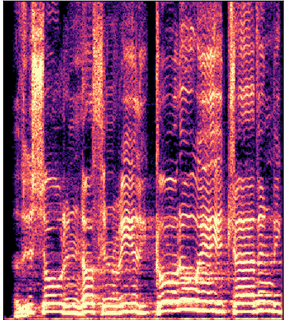
\includegraphics[width=0.3\textwidth]{frontmatter/TitleSpectrogram.png}
  \vspace*{2cm}
  \begin{center}
    \begin{Huge}
      \@title
    \end{Huge}\\[0.1cm]
    \vspace*{1cm}
    \begin{Large}
      \@subtitle
    \end{Large}\\
    %
    \emph{by}\\
    \@author \space \space 30748119
    %
    \vfill
    A document submitted in partial fulfillment
    of the requirements for the degree of\\
    \emph{Aeronautics and Astronautics}\\
    at\\
    \textsc{University of Southampton}\\
  \end{center}
  \makeatother
\end{titlepage}

\newpage
\null
\thispagestyle{empty}
\newpage

\begin{center}
  \textsc{Abstract}
\end{center}

\noindent

In this thesis, a deep learning architecture called DDSP is used for synthesizing realistic vocal features. DDSP is a collection of machine learning models, differentiable versions of standard digital signal processing elements such as oscillators, noise filters, and other valuable tools for learning how to decode, learn and subsequently synthesize new musical audio signals.

The DDSP architecture is applied to a set of vocal samples of two different artists' voices to create a model for each respectively. The models extract pitch, amplitude, and timbre information from the vocal samples. Several inferencing tests are then conducted to determine the performances of the trained models at various tasks.

Finally, the results are concluded, and areas for improvement for future work are suggested.
\begin{center}
    \textsc{Declaration}
\end{center}

I, Harry Twigg, declare that this thesis and the work presented in it are my own and have been generated by me as the result of my original research. I confirm that:

\begin{enumerate}
    \item This work was done wholly or mainly while in candidature for a degree at this University
    \item Where any part of this thesis has previously been submitted for any other qualification at this 
    University or any other institution, this has been clearly stated
    \item Where I have consulted the published work of others, this is always clearly attributed
    \item Where I have quoted from the work of others, the source is always given. Except for such
    quotations, this thesis is entirely my work
    \item I have acknowledged all main sources of help
    \item Where the thesis is based on work done by myself jointly with others, I have made clear exactly what 
    was done by others and what I have contributed myself
    \item Where open source software has been used, I have abided by the license agreement that was provided with the software and made any derivative work publicly available under the same license
    \item None of this work has been published before submission unless indicated.
\end{enumerate}

%  \begin{center}
    \textsc{Acknowledgements}
\end{center}

I want to thank my supervisor, Professor Thomas Blumensath, for his support and guidance during my project. He let me go beyond the project's initial scope and into an area I honestly found very exciting whilst also keeping me on track with the project's original goals.


\begin{center}
    \textsc{Supplementary Information}
\end{center}

This thesis contains accompanying code and audio files not included in the thesis itself. It is recommended that listening to these is done while reading the experimental results.

These can be found in the following public GitHub repository:

\href{https://github.com/harrytwigg/FEEG3003}{https://github.com/harrytwigg/FEEG3003}

Open source code licenses used in this code can be further found at the end of this paper in the section \nameref{chapter:open_source_licenses}

\tableofcontents


\cleardoublepage
\phantomsection
\addcontentsline{toc}{chapter}{\listfigurename}
\listoffigures

\mainmatter

\chapter{Introduction}

\noindent Teaching a computer to synthesize music using deep learning based methods has historically been a difficult task. Audio contains thousands of sound features every second in the time domain that are difficult to accurately teach to a neural network. Even if a network successfully learns how to interpret musical features, the output of models often sound fake or jarring to the listener due to inaccurate pitch and timbre representations and a lack of temporal context.

A subset of this topic is vocal sound synthesis using neural networks. This niche pertains to synthesizing singing and speech sounds using deep learning methods. This has historically proven more difficult than synthesizing instrumental based music due to the complexity of the human voice, with many different vocal modes and features that are difficult to learn through a neural network.

In this paper, the problem of difficulty surrounding synthesizingn the human voice and singing is investigated. A variety of approaches have been proposed to solve this problem, with varying degrees of success, the methods and the results of which are discussed in this paper.

The goal of this paper is to compare the various approaches to vocal sound synthesis, evaluating the merits and limitations of each approach. With the ultimate goal of building on the best of the existing methods further, demonstrating the applicability of the proposed approach.

Many potential applications would be oppened up if a deep learning model could be devised that could accurately learn, understand, and synthesize the fundamental features of music. These uses include many potentially artistic and business applications:

\begin{itemize}
    \item Rapidly generating new music
    \item Pitch transposing a piece of music eg transposing a piece of music down an octave, or up an octave.
    \item Changing room accoustics, eg if a piece of music was played in any echoic room, the model could be used to re-synthesize the same piece of music in an anechoic environment.
    \item Change the singing voice in a particular piece of music, in a similar fashon to deepfakes.
    \item Musical remixes of existing songs with different singers.
    \item Potentialy brand new forms of artistic expression, with a neural network perhaps being able to produce vocal features that are impossible to create naturally.
\end{itemize}

\section{Aim}

This paper aims to evaluate the many approaches to music sound synthesis, with an aim to build on the most promising approach further, applying it to a music sound synthesis problem, demonstrating its effectiveness.

\section{Objectives}

\begin{enumerate}
    \item To evaluate existing approaches to vocal audio signal encoding and sound synthesis using deep learning methods.
    \item Build on the best of the existing methods of vocal audio signal encoding and sound synthesis, validating and demonstrating the applicability of the proposed approach to the music sound synthesis problem.
    \item Derive constructive reccomendations for future research based on the research undertaken.
\end{enumerate}

\section{Methodology}

A standardised process was developed to evaluate the quality of existing methods, and a critical review of existing literature on music sound synthesis (focusing on vocal sound synthesis) was conducted. This standardised process was necessary as it would be difficult to compare the results of different methods. Each of the approaches evaluated used different levels of abstraction and resolution of musical and audio data. Additionally, they have different trade-offs in terms of accuracy and computational efficiency.

The standardised process is based on good machine learning principles and academic best practices. The technical requirements are as follows:

\subsection{Technical Requirements}

\begin{itemize}
    \item Overly time-consuming methods should be penalised due to the limited time for the project. These can come in many forms, e.g. excessive training and computation time or extensive datasets requirements, excessive hyperparameter tuning, or overly large networks
    \item Use of teacher forcing or operator involvement in any methods. Teacher forcing leads to biases in the model outputs and limits the scalability and ease of using any derived models. Manually labelled data shall also be penalised similarly.
    \item Poor tonal quality in the output, e.g. it is noticeable that the model was generated digitally instead of recorded. Poor tonal quality could be caused by:
          \begin{itemize}
              \item Spectral leakage due to inaccuracies in Fourier representations
              \item Poor oscillatory output representation that sounds synthetic
          \end{itemize}
    \item To analyse the tonal quality, a statistical method of loss must be defined and used
    \item Modular systems shall be evaluated positively because their elements can be built on separately, and the whole system acts less like a 'Black Box'.
    \item Any discarded information, e.g. phase that has been discarded during encoding (e.g. phase) that could be presented to the network shall also be penalised. It is hypothesised that this information could be used to improve the quality of the output.
    \item Model architectures specific to music and audio signal processing were preferred instead of more general ones. Furthermore, it was believed that directing the model towards specific musical features (such as harmonics and pitch) would be beneficial, rather than generalising to the entire audio signal.
\end{itemize}

\subsection{Academic Requirements}

Well cited papers or those in scientific journals were looked upon favourably, showing that other people have found the work valuable and, more importantly, credible. It was also desired that any researched papers have open-sourced code and that the code is available for use. Without this, the model cannot be quickly built without building the codebase from the ground up, which would take considerable time. Older methods that have not been built further were evaluated negatively, as this suggests that experts in the field have judged the work to be of no further benefit and hence obsolete.

\subsection{DDSP Training}

After the initial research, DDSP, a modular approach, was picked; it enabled modification of evaluated sound qualities called latents (pitch, loudness) and a series of differentiable versions of traditional signal processing techniques. DDSP was the most promising model architecture due to several factors discussed in \nameref{section:DDSP}.

Two different datasets were created, one male voice artist and one female voice artist, to see how the DDSP architecture would handle male and female voices differently.

For each artist, two different albums were picked of similar musical styles to ensure consistency of vocal style across the entire dataset; this was done to try and encourage the model to learn a specific timbre of voice.

The albums were picked so that they only had one voice on the vocal track to avoid any problems of the model mixing voices, any songs with cover artists or different singers to the leading voice were removed.

Each dataset was processed through a pre-trained model called Spleter\cite{Spleeter}. This pre-trained model separated the vocal track from the instrumentals for each song in the album. Consequently, large datasets could be easily created featuring a singular vocal track and enabling datasets 10x the size of the paper this work was based on\cite{SingingDDSP}.

Each dataset was then trained using the DDSP library\cite{DDSPPip} and code adapted from a variation of DDSP designed for singing\cite{SingingDDSP}. Model hyperparameters were kept the same as in the Singing DDSP paper\cite{SingingDDSP} as the researchers had demonstrated thorough testing of which hyperparameters were the best. 200,000 epochs were used for each dataset; this was deemed sufficient for this project whilst keeping the training time manageable.

\subsection{DDSP Inferencing}

Following the training of both models, the models underwent several inferencing tests designed to evaluate the models' encoding of the latent characteristics.

\begin{enumerate}
    \item The models were inferred on the same dataset used for training to test the model's accuracy in predicting frames from the training dataset.
    \item A pitch transposition was attempted. Vocal samples from the original dataset were transposed up and down an octave to see how the model would perform on unseen vocal ranges.
    \item A mono-pitch inference test was conducted to determine the model's ability at producing a single pitch.
    \item A log-linear loudness inference was attempted to gauge the model's ability to modify the loudness of the vocal samples.
    \item For the best dataset, two unseen vocal tracks of different artists were put into the model to see how the model would perform on unseen vocal samples of different artists to gauge the model's generalisation ability to other artists and unseen vocal types.
\end{enumerate}

Finally, in light of the experimental results and other academic research, recommendations for future work in the field are made.

% TODO: Move to literature review or later sections

%Additionally the model could be accurately trained on smaller datasets with smaller model sizes, reducing the training cost and time assocciated with certain model accuracy.
%
%Most DDSP research to date has been focused on modelling of musical instruments, this is due to their relative constant timbre characteristic over an entire instrument, making it easier to model.
\chapter{Literature Review}

\begin{center}
    \begin{minipage}{0.5\textwidth}
      \begin{small}
        The evaluation of all the literature on vocal sound synthesis methods is undertaken here, they are laid out in a roughly chronological order. DDSP is outlined in the greatest depth as it was the technique chosen for further investigation.
      \end{small}
    \end{minipage}
    \vspace{0.5cm}
  \end{center}

\section{Symbolic Methods}

Using computers to generate music is a vast field of research dating almost as far back as the invention of computers themselves\cite{Hiller1958Musical}. However, the first research into using machine learning to generate music goes back to the 1980s\cite{ConnectionistComposition}\cite{GradientDescentLearning} with the very first research on symbolic data. These higher-level representations often took the form of MIDI or other musical notation.

Symbolic based models provide a high-level abstraction of the musical piece, meaning that they are easier to train as the model does not have to worry about the physical process to produce sound. However, they are significantly limited to music that can be described in midi notation, i.e. vocals and other instruments with unique modes of being played cannot be used. One paper proposed using an autoregressive recurrent neural network to generate symbolic music. Many later works build on Recurrent Neural Networks.

More recent works in the field are symbolically applying new modern transformer machine learning architectures to generate music with long-term structurework\cite{LongTermStructure}; this is a challenge experienced in many music synthesis models. Transformer based architectures do not rely on recurrent or convolutional based mechanisms and instead use what is called an attention-based mechanism to generate long term structure\cite{Attention}.

\subsection{Critical Evaluation}

Due to their high level of abstraction, Symbolic methods have smaller models with fewer parameters and are easier to train. As a result, they prove helpful in generating abstract long term musical structures. Furthermore, the relatively recent papers showing long term structure\cite{LongTermStructure} and the use of an attention mechanism\cite{Attention} have shown that symbolic methods have future potential and relevance.

Nevertheless, symbolic methods have low levels of resolution and can only be used to generate music described in terms of midi or similar notation. This limited expression is a limitation of symbolic methods, as they cannot be used to generate raw time-series audio features. Furthermore, they have no way of generating the intricacies and expression of the human voice; this is hard to describe symbolically. 

Sadly the disadvantages of symbolic methods (specifically their lack of output expression) outweigh any benefits they offer in forms of long term musical structure. Nevertheless, even if they are limited in their range of expression, they could be helpful if combined with another model capable of synthesizing time-series audio data. The symbolic model could provide the other model with a long term musical structure, and the other model could generate local audio time-series audio.

\section{Raw Waveform Based Encoding}

A subset of deep learning research has focused on waveform-based methods and encoding music audio directly as raw time-series audio data.

There are many potential benefits to crunching low-level audio data. Firstly, information discarded from spectrograms, e.g. phase, is not lost. Secondly, using raw audio does not limit the number and depth of features that can be learned, meaning such a model could potentially learn the intricate features of the human voice.

One of the problems of waveform based models is their lack of long term structure; this is caused by the sampling period being so short and the many thousands of samples that make up one continuous raw audio track\cite{JukeboxWebsite}.

\subsection{Jukebox}
\label{sec:jukebox}

The most influential model employing waveforms for music sound synthesis is called Jukebox\cite{Jukebox}. The Jukebox model is a deep neural network that learns to reconstruct music's vocal (and instrumental features) features from the raw audio data.

What is significant about the paper is its method of attempting to overcome the lack of long term structure. An autoencoder compresses input raw audio at the Nyquist Frequency to a discrete space using a technique called Vector-Quantized Variational Autoencoders (VQ-VAE)\cite{Jukebox}.

\vspace{0.5cm}
\framebox[1.1\width]{
    \begin{minipage}{0.8\textwidth}
        The Nyquist frequency is the highest frequency that can be represented by a sampling rate of an encoded audio signal so that the original signal can be reconstructed\cite{ProbabilityAndStatistics}.
    \end{minipage}
}
\vspace{0.5cm}

Several independent VQ-VAE Levels are used, retaining different levels of resolution up to 128x encoding. Lower levels capture local music structures, e.g. timbre and local pitch, whereas higher levels capture higher-level long-range music structure features.

Each level is then trained using sparse transformer-based models to learn the probability distribution of the VQ-VAE at each level of resolution.

\begin{figure}[H]
    \centering
    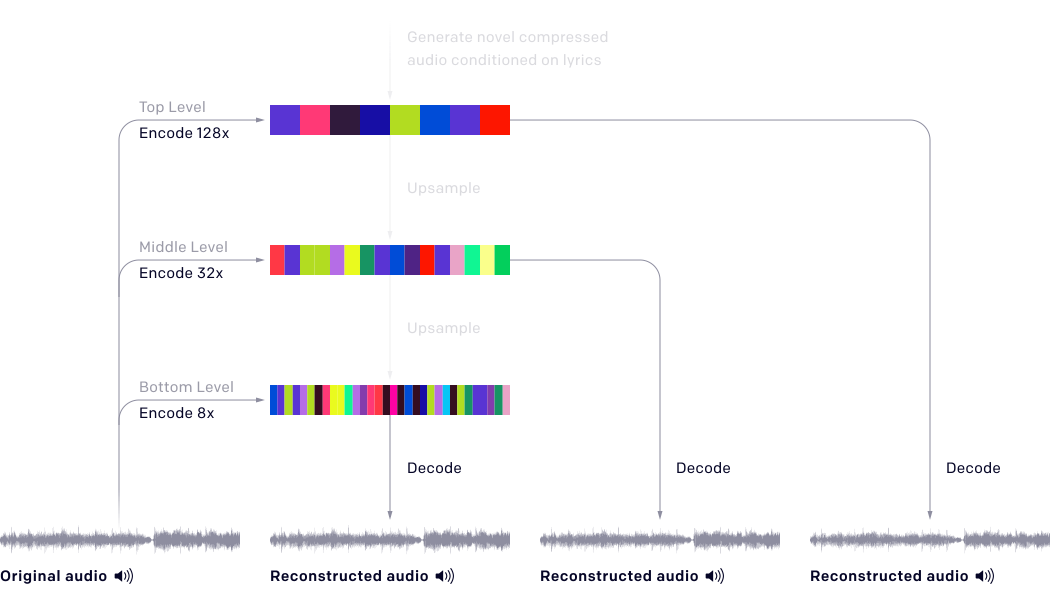
\includegraphics[width=0.8\textwidth]{literature_review/vq-vae.png}
    \caption{VQ-VAE Encoding and Compression: Successive levels further compress the raw audio data, discarding irrelevant information}
    \label{fig:jukebox_example}
\end{figure}

\subsection{Critical Evaluation}

The Jukebox model can be conditioned on lyrics, genre, and artist. After training, new songs can be upsampled through each level of VQ-VAEs to give new raw music audio. Outputted music features singing, instrumentals and some resemblance to a long-term structure. Music vocals are also synthesised and sung by the model on its own accord.

Although local musical coherence and timbre are good in Jukebox, the longer-term musical structure is not fully present. The upsampling process also introduces significant noise into the final audio, which sounds jarring to the listener. Another significant disadvantage is the lack of parallel sampling and the autoregressive nature of the model, meaning it takes multiple hours to produce one minute of music. This slowness limits its broad applicability as it is prohibitively expensive and prevents real-time applications. The model also functions much like a black box, preventing us from gaining any critical information about how it is synthesising its audio. This further limits its potential uses as we cannot independently modify model parameters such as the pitch and timbre of generated music. Finally, waveform based models require significant training data to train the model and extract relevant musical features accurately.

Sadly the lack of real-time features and prohibitively large model size from using raw time-series based encoding. As per the technical requirements, any real-world application needs to be real-time or near-realtime.

\section{Fourier Methods and Spectrograms}

Spectrograms have a long history but were first used with machine learning models to synthesise music at the start of the 21st century\cite{NoteOnsetDetection}.

The time-domain based audio signal was divided into equal lengths of shorter periods. Then, a Fast Fourier Transform (FFT) is applied to each segment, decomposing the signal at each of the timestep periods into its constituent frequencies and corresponding amplitude. The complex values from the Fast Fourier Transform are complex values, giving spectrograms of frequency and phase.

A spectrogram is a graphical plot of the decomposition of sound using the \acrfull{STFT}. It consists of 2 plots frequency against time and phase against time. Each point of the plots is coloured in amplitude/intensity of the decomposed audio signal at a specific point in time. The STFT is a sum of overlapped Fast Fourier Transforms (FFTs) of the audio signal. After calculation of the STFT, the sample is divided into overlapping frames of equal length, known as the hamming window. Finally, the FFT is then applied to each audio signal frame. The outputted complex functions from the Fast Fourier Transform give spectrograms of amplitude and phase of different frequencies at each timestep.

\subsection{Mel-Spectrograms}

Mel Spectrograms are an adaptation of the spectrograms more suited to sounds intended to be heard by humans. Mel Spectrograms have amplitude/sound intensity adjusted along a logarithmic scale such that graphical distances between frequencies sound the same distance as human hearing would detect them to be. This adjustment enables machine learning models to learn how to produce audio sequences that sound more natural to a human listener.

\begin{figure}[H]
    \centering
    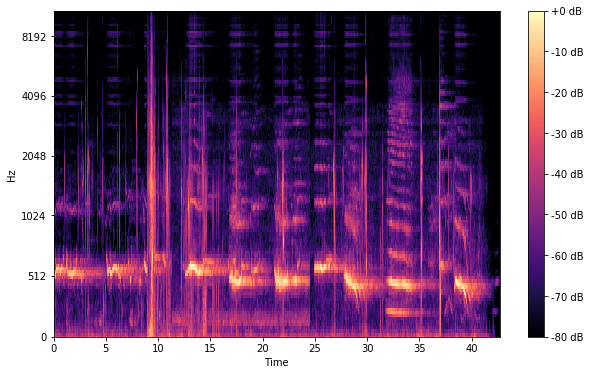
\includegraphics[width=0.8\textwidth]{literature_review/MelSpectrogram.png}
    \caption{An example of a  Mel Spectrogram showing the amplitude of different frequencies in a sound over time\cite{GettingToKnowTheMelSpectrogram}}
    \label{fig:spectrograms}
\end{figure}

There is no standardised formula for converting frequncy onto the mel logarhthmic scale as it is up to interpretation the adjustment level that is required for human hearing, though then most common formula is\cite{SpeechCommunication}:

\begin{equation}
    m = 2596 log(1 +  \frac{f}{700}) = 1127 ln (1 + \frac{f}{700})
\end{equation}

\subsection{Intepreting Phase}

The STFT is a complex function; however, only the magnitude part is currently utilised by most models, and the phase part is discarded. Phase is key to interpreting musical sounds; without it, synthesised sounds can sound unnatural as signal information is discarded.

Success at interpreting the phase spectrogram to date has been limited. As a result, most models discard the phase part of the signal and make models purely off the frequency spectrogram. Discarding the phase is a problem as the phase is a crucial part of spectrogram representation, making the image representation fully convertible back to audio, though it is challenging to work with for several reasons:

Firstly, the phase spectrogram appears random, making it challenging to distinguish meaningful information from noise.

Secondly, the spectrogram phase is a cyclic quality. Cyclic qualities are more challenging to interpret than non-cyclic qualities as they are not continuous. One paper called GANSynth\cite{GANSynth} overcomes this problem by calculating the phase difference between individual timesteps of a spectrogram and making $2\pi$  adjustments for when the phase wraps around. This phase difference is called the instantaneous frequency and provides far more informative information than the raw phase. Instantaneous frequency over harmonics, for instance, is expected to be constant.

\begin{figure}[H]
    \centering
    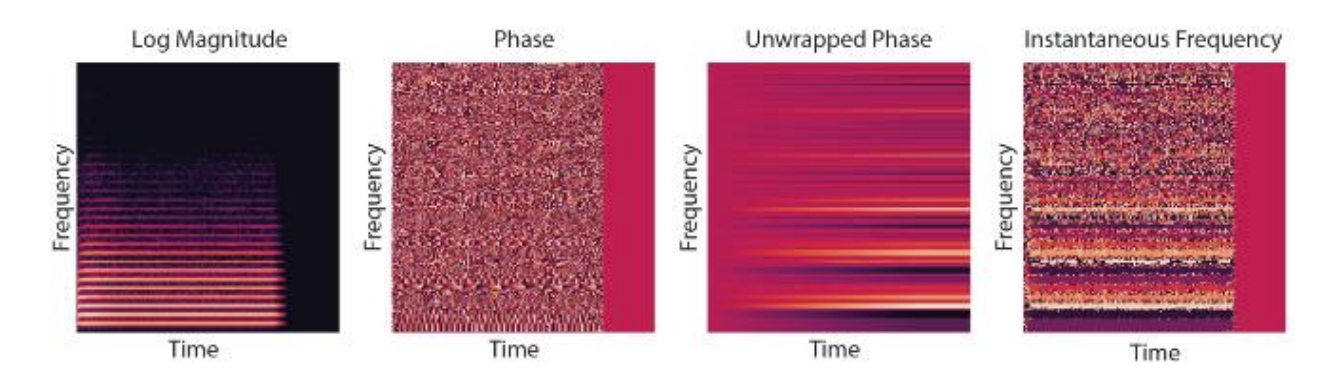
\includegraphics[width=0.8\textwidth]{literature_review/PhaseAdjustment.png}
    \caption{Unrwapping Spectrogram Phase: An illustration from the GANSynth paper of how the phase of a spectrogram is adjusted to make it more interpretable to a neural network\cite{GANSynth}}
    \label{fig:phase_unwrapping}
\end{figure}

\subsection{Spectrogram Evaluation}

Spectrogram based encoding for music sound synthesis is currently the best method for encoding musical sounds due to their ease of use and the low-level control over signal information that does not hinder their interpretation (unlike raw waveform encoding). Conventional image processing models, e.g. Convolutional Neural Networks or Recurrent Neural Networks, can be used to process the spectrogram. These models can extract local sounds at specific frequencies from a spectrogram and learn how to reproduce them. This extraction is possible due to the separated frequency and timewise position of sounds that form specific image patterns that an autoencoder can be trained to recognise. An example in this case of singing is shown in the following Figure \ref{fig:spectrogram_features}:

\begin{figure}[H]
    \centering
    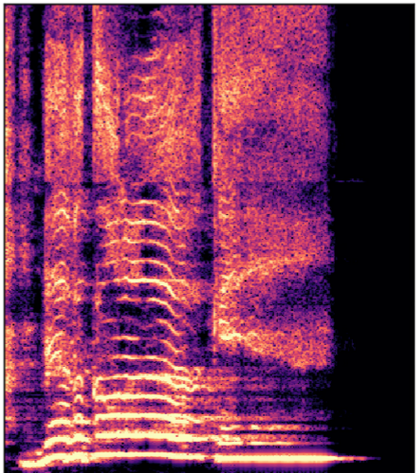
\includegraphics[width=0.4\textwidth]{literature_review/SpectrogramFeatures.png}
    \caption{Spectrgram Features: Regular harmonics present in singing can be observed in the bright horizontal regions of the spectrogram that repeat at regular frequency intervals. A model could be trained to extract these features and learn to resynthesize them}
    \label{fig:spectrogram_features}
\end{figure}


Additionally, one of their defining advantages is that they can be used to reconstruct the original audio signal from the spectrogram with the inverse Fourier Transform. The reconstructed audio signal will be almost identical to the original (phase-matched) if phase and magnitude spectrograms are used.
Spectrograms are at the core of many recently published music synthesis models and papers, showing academic relevance.

However, most models based on spectrograms, e.g. raw CNN-based models, are limited and do not make use of biases in sound, for instance, the tendency of natural sounds to oscillate sinusoidally at harmonic frequencies according to the harmonic plus noise model. In addition, many traditional autoencoder-based RNN models do not enable the configuration of specific sound features, e.g. fundamental frequency or loudness. Additionally, spectrogram based models are not without problems (e.g. the discarding phase of information).

Therefore spectrograms, although helpful, cannot be used to synthesise audio signals on their own; to achieve widespread academic and commercial use, a different representation to help a model relate them to sound is required, for example, \nameref{section:DDSP}.

\section{Differentiable Digital Signal Processing}
\label{section:DDSP}

Differentiable Digital Signal Processors (DDSP) are differentiable versions of traditional digital signal processing elements (such as harmonic oscillators and filtered noise banks) that can be integrated into machine learning models\cite{OriginalDDSP}. They are a relatively novel invention but build on the foundations of traditional spectral encoding and modelling techniques such as Mel-Spectrograms and Fourier transforms. Although they were designed to model musical instruments, they can be extended to the human voice.

The DDSP network is modular and consists of multiple separate feedforward components (featuring a separate encoder and decoder) instead of a single recurrent based network. Information is fed between the encoder and decoder in time-dependent information called latents; these are fundamental frequency and loudness.

The model aims to take advantage of what the authors call inductive biases of sound instead of making the model figure out all the features of sound itself. This idea is well validated and is known as the harmonic plus noise model of spectral modelling synthesis\cite{HarmonicPlusNoise}. For example, an instrument's track could have harmonic vibrations at multiples of the fundamental frequency and noise components coming from a white noise source through a series of filter banks that change over time.

\subsection{Spectral Modelling Synthesis}

DDSP synthesiser elements are based on traditional synthesiser-based components that can be combined with an encoder and decoder to form a complete machine learning model. DDSP uses a type of sound modelling called Spectral Modelling Synthesis\cite{SpectralModellingSynthesis} to model sound, with the components being modified, so they are differentiable. By recreating them as differentiable components, the gradients of each block can be accessed in the machine learning model, enabling them to be configured by the model. Synthesisers take the network outputs of the decoder and use them to synthesise an output audio signal.

\subsubsection{Harmonic Oscilator}

The harmonic oscillator is the first of the 2 Spectral Modelling Synthesis components. It consists of a bank of oscillators that output a sinusoidal signal denoted as $x(n)$ where $n$ represents discrete time steps and is equal to the sum of the sinusoidal waves. The harmonic oscillator can be expressed as:
\
\begin{equation}
    x(n) = \sum_{k=1}^{N} A_k(n) \sin(\phi_k(n))
\end{equation}

\begin{itemize}
    \item $x(n)$ is the output signal
    \item $A_k(n)$ is the amplitude of the kth sinusoidal oscillator
    \item $\phi_k(n)$ is the instantaneous phase of the kth sinusoidal oscillator
\end{itemize}

The phase at a certain point in the output signal can be calculated as follows using the instantaneous frequency:

\begin{equation}
    \phi(n) = 2\pi\sum_{m=0}^N f_k(m) + \phi_{0,k}
\end{equation}

\begin{itemize}
    \item $\phi_k(n)$ is the instantaneous phase of the kth sinusoidal oscillator
    \item $f_k(m)$ is the instantaneous frequency of the kth sinusoidal oscillator
    \item $\phi_0(k)$ is the initial phase of the kth sinusoidal oscillator
\end{itemize}

Like actual sound, each harmonic oscillator's frequency $f_k(m)$ is an integer multiple of the fundamental frequency $f_0(n)$. For example the kth harmonic oscillator, the instantaneous frequency is defined as:

\begin{equation}
    f_k(m) = k \times f_0(n)
\end{equation}

The highest harmonic should be at the Nyquist frequency, which is half the sample rate or mathematically as:

\begin{equation}
    f_{Nyquist} = N \times f_0(n)
\end{equation}

Defining the highest harmonic in this way ensures that the harmonic oscillator can represent all of the possible signal ranges.

The initial phase $\phi_0(k)$ can be random, fixed or learned\cite{OriginalDDSP}.

DDSP employs bilinear interpolation upon the fundamental frequency to increase the sample rate from that of the neural network and smoothing to prevent artefacts. Bilinear interpolation is necessary as the neural network is trained at a lower sample rate than the original signal whereas oscillators operate at the original sample rate.

\vspace{0.5cm}
\framebox[1.1\width]{
    \begin{minipage}{0.8\textwidth}
        Bilinear interpolation is a mathematical technique enabling the estimation of new values between existing discrete values that are the functions of two variables. In DDSP, it is used to increase the neural network's sample rate to that of the underlying audio signal.
    \end{minipage}
}
\vspace{0.5cm}

\subsubsection{Filtered Noise}

The filtered noise is a component of the DDSP synthesiser. For example, white noise is filtered by a \acrfull{LTI-FIR} to produce a noise signal. LTV-FIR filters are a type of filter that can vary over time, enabling different noise patterns to be generated at different time steps in the output signal.

Finite impulse response filters consist of mathematical impulse responses, meaning that the filter is of finite duration, enabling the filter to change and, over time, model different stochastic noises in the output signal.

As the filters are linear time-invariant, the noise filter can be characterised by its response to different frequencies of sinusoids, known as its frequency response. The filter is also independent of time.

It is worth noting that the noise filter is applied in the frequency domain; this is done to avoid phase distortion. Phase distortion occurs when a filter's phase response is not linear in the frequency domain. A lack of linearity in the filter domain can distort the filter's output, making synthesised sounds sound unrealistic.

The neural network was tasked with predicting frequency domain transfer functions of the filter for every frame of the output signal, denoted as $H_l$\cite{OriginalDDSP}.

For all notations with subscript l, l denotes that the values are for the lth frame of the output signal.

$H_l$ is in the frequency domain; it shows the filter's frequency response. Even though LTV-FIR filters are not linear time-variant, the network can vary the FIR filter over time, allowing the filter to change over time for modelling different noise patterns.

As linear time-invariant filters can be denoted by their impulse response, the frequency response of the filter can be denoted by its impulse response $h$, as shown below:

\begin{equation}
    H_l = \mathscr{F}^{-1}(h_l)
\end{equation}

\begin{itemize}
    \item $H_l$ is the frequency response of the filter in the frequency domain
    \item $h$ is the impulse response of the filter
    \item $\mathscr{F}^{-1}$ is the inverse descrete Fourier transform
\end{itemize}

In order to apply the time-varying filter to map the input to the output, the following is done:

\begin{enumerate}
    \item An input white noise signal is split into non-overlapping frames of fixed hop size, each one to go with a certain impulse response $h_l$.
    \item Frames are then multiplied in the fourier domain: \begin{itemize}
        \item $Y_l = H_l X_l$
        \item $Y_l$ is the output signal, where $X_l = \mathscr{F}(x_l)$, where $\mathscr{F}$ is the \acrfull{DFT}
        \item $X_l$ is the input signal, where $Y_l = \mathscr{F}^{-1}(y_l)$, where $\mathscr{F}^{-1}$ is the \acrfull{IDFT}
    \end{itemize}
    \item Output audio frames are then retrieved using the inverse Fourier transform:
        $y_l = \mathscr{F}^{-1}(Y_l)$
    \item Output audio frames are then comnbined, using the same hop size as the input audio frames.
\end{enumerate}

\vspace{0.5cm}
\framebox[1.1\width]{
    \begin{minipage}{0.8\textwidth}
        Hop size refers to the number of samples between each frame; the number of samples in a frame equals the hop size.
    \end{minipage}
}
\vspace{0.5cm}

The filtered noise synthesiser can generate many different noise patterns that are not harmonic and continuous. The original DDSP authors used them to generate unique instrument features, such as the plucking of a violin, but they can also be used to generate consonants in the human voice \cite{SingingDDSP}.

\subsection{Model Setup}

\begin{figure}[H]
    \centering
    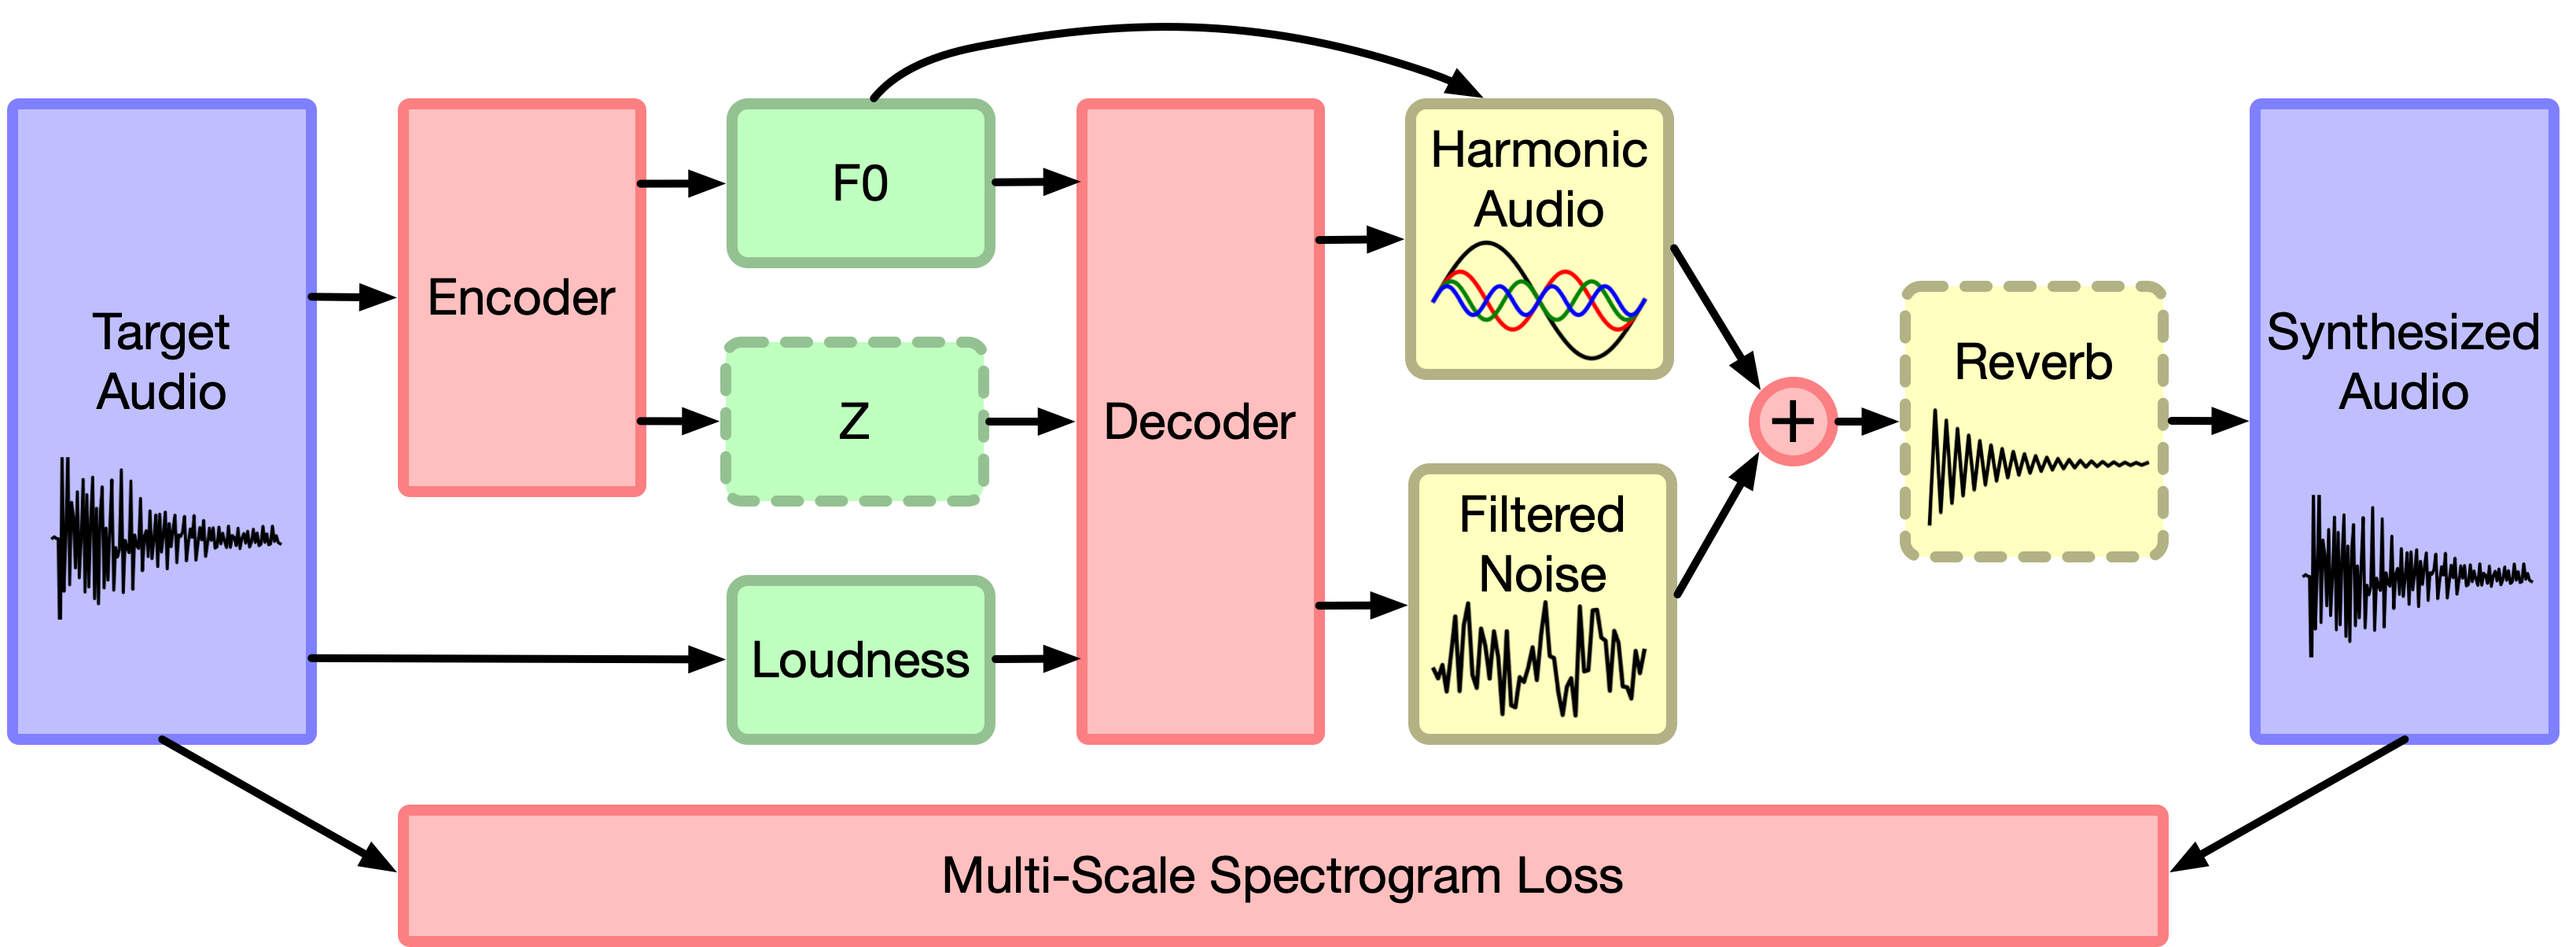
\includegraphics[width=0.8\textwidth]{literature_review/DDSPArchitecture.png}
    \caption{The DDSP Model Architecture: The model setup courtesy of a DDSP paper\cite{SingingDDSP}. Standardised machine learning components are shown in red, the latent variables in green and the synthesizers in yellow. Note the feed-forwarding of F0 bypassing the decoder to directly control the harmonic oscillators.}
    \label{fig:ddsp_model_setup}
\end{figure}

The harmonic oscillators and filtered noise are combined to produce the synthesised output signal in what is known as the Harmonic plus Noise model. The combined output can also be passed through additional modules to produce different types of sounds, for example, a reverberation module to accurately model the acoustic characteristics of a string instrument; this is, however, beyond the scope of this paper. No reverb or additional modules are included in this thesis.

The initial DDSP model\cite{OriginalDDSP} employed a modified autoencoder decoder setup where the autoencoder was trained to minimise reconstruction loss in an outputted synthesised audio. Training data is fed into the encoder in the form of Mel-spectrogram images. The autoencoder attempts to extract information from the input signal. F0 is directly fed into the harmonic oscillators as making them learn to reproduce this would be unnecessary.

A further latent quality called Z is extracted from the output of the encoder representing the outputs of the encoder, this cannot be modified, it is fed directly into the decoder. The original DDSP paper demonstrated that timbral information was encoded in this latent Z, enabling timbral transfer between various musical instruments to be possible.

Loudness and fundamental frequency, and Z are time-dependent, they can be denoted as such: $f(t), l(t), z(t)$.

F0, the fundamental frequency, can extracted using an encoder in the standard mode. The DSP architecture is however, very flexible. Therefore, different variations of this autoencoder setup can be used. For example, instead of forcing the encoder to map F0, CREPE can be used to extract the F0 from the input signal.

\vspace{0.5cm}
\framebox[1.1\width]{
    \begin{minipage}{0.8\textwidth}
        CREPE is a highly accurate pitch detection based \acrfull{CNN}\cite{CREPE}. It can accurately predict pitch with an accuracy of over 99.9\%. In addition, it is a pre-trained model that can be used with the DDSP library to extract the pitch from the input signal accurately.
    \end{minipage}
}
\vspace{0.5cm}

The decoder then uses the F0, latnet Z, and the statistically determined loudness to derive control values for the filtered noise and oscillator synthesisers, learning how to re-synthesise the target-audio track.

The fundamental frequency is, however, additionally fed directly into the synthesisers as it enables the model to respond to frequencies unseen during training\cite{SingingDDSP}.

Due to the modular design, certain features can be explicitly controlled, for example, room acoustics. Some networks would implicitly pick up room acoustics. This method may introduce unnecessary mode covering, increasing potential training time. The DDSP model explicitly defines room acoustics using a reverberation synthesiser (see Figure \ref{fig:ddsp_model_setup}).

\subsection{Measure of Loss}
\label{sec:loss_measure}

In order to train the model, it is necessary for a measure of loss to be defined. The autoencoder is tasked with minimising the reconstruction loss; this is the difference between the synthesised audio and the target audio. Unlike in a conventional autoencoder model, the loss cannot be defined pointwise as two waveforms may sound the same but have different pointwise characteristics. The loss function is therefore defined using a method called multi-scale spectral loss. The loss is defined as the sum of L1 differences and the L1 log difference between the target and synthesised magnitude spectrograms.

\vspace{0.5cm}
\framebox[1.1\width]{
    \begin{minipage}{0.8\textwidth}
        L1 loss is defined as the sum of the absolute differences\cite{L1Statistic}, the sum of the absolute differences between the magnitude spectrograms.
    \end{minipage}
}
\vspace{0.5cm}

\begin{equation}
    L_i = ||S_i - \hat{S_i}||_1 + ||\log{S_i} - \log\hat{S_i}||_1
\end{equation}

\begin{itemize}
    \item $L_i$ is the model loss FFT of size $i$
    \item $S_i$ is the target spectrogram with a given FFT of size $i$
    \item $\hat{S_i}$ is the synthesized spectrogram with a given FFT of size $i$
    \item $||S_i - \hat{S_i}||_1$ is the L1 difference between the target and synthesized spectrograms
    \item $||\log{S_i} - \log\hat{S_i}||_1$ is the L1 difference between the target and synthesized logarithmic Mel-spectrograms
\end{itemize}

The total loss is then equal to the sum of spectral losses for different FFT sizes:

\begin{equation}
    L = \sum_{i=1} L_i
\end{equation}

Where $i \in (4096, 2048, 1024, 512, 256, 128, 64)$

\subsection{Speech Synthesis Using DDSP}

Further research on top of DDSP relating to vocals has been done for speech synthesis, although not directly designed for music; the paper introduces a slightly different system that modifies the DDSP architecture to more closely match the human voice\cite{SpeechDDSP}. Instead of using an autoencoder, the network uses a series of convolutional neural networks.

The method yields highly accurate results (although it is still noticeable that the output has been synthesised). Timbre was accurately measured, though consonants still sounded off. Unfortunately, the code used for the model was not available for download, limiting the value of the paper as its findings could not be replicated. It could, in theory, be reversed engineered though this would take considerable time and effort and is, as such, beyond the scope of this project. It is also possible that the results were cherry-picked from the original as only a limited number of samples were available.

\subsection{Singing Voice Synthesis Using DDSP}
\label{sec:singing_voice_synthesis}

A new team has conducted attractive work building on top of the initial paper to produce singing voice synthesis\cite{SingingDDSP} specifically. This paper outlines how the DDSP model can be further altered to interpret better and learn how to model the human voice.

The adaptation involved adding \acrfull{MFCC} an additional time-varying form of encoding. The coefficients together make up a \acrfull{MFC}. A Mel-frequency cepstrum (MFC) represents the spectrum of a signal using a non-linear Mel frequency scale.

MFFCs have a long history of use in telecommunications and speech processing\cite{MFCCHistory}. Thus, the original authors hypothesised that this representation would more accurately model the non-linearity of the human voice, thus making a vocal synthesis model more accurate.

The modified decoder and MLP can be seen in Figure \ref{fig:singing_decoder_mlp}. An additional MLP layer has been added to the decoder to allow for the MFC to be learned. Besides this addition, the DDSP architecture is the same as the original, continuing to rely on the harnonic plus noise model.

\vspace{0.5cm}
\framebox[1.1\width]{
    \begin{minipage}{0.8\textwidth}
        Multilayer Perceptron (MLP) is a feedforward neural network module. MLPs feature a directed graph, meaning that the signal path only goes one way. Each node is also characterised by a non-linear activation function. Here the MLP is used to learn the Mel Frequency Cepstrum and its coefficients.
    \end{minipage}
}
\vspace{0.5cm}

\begin{figure}[H]
    \centering
    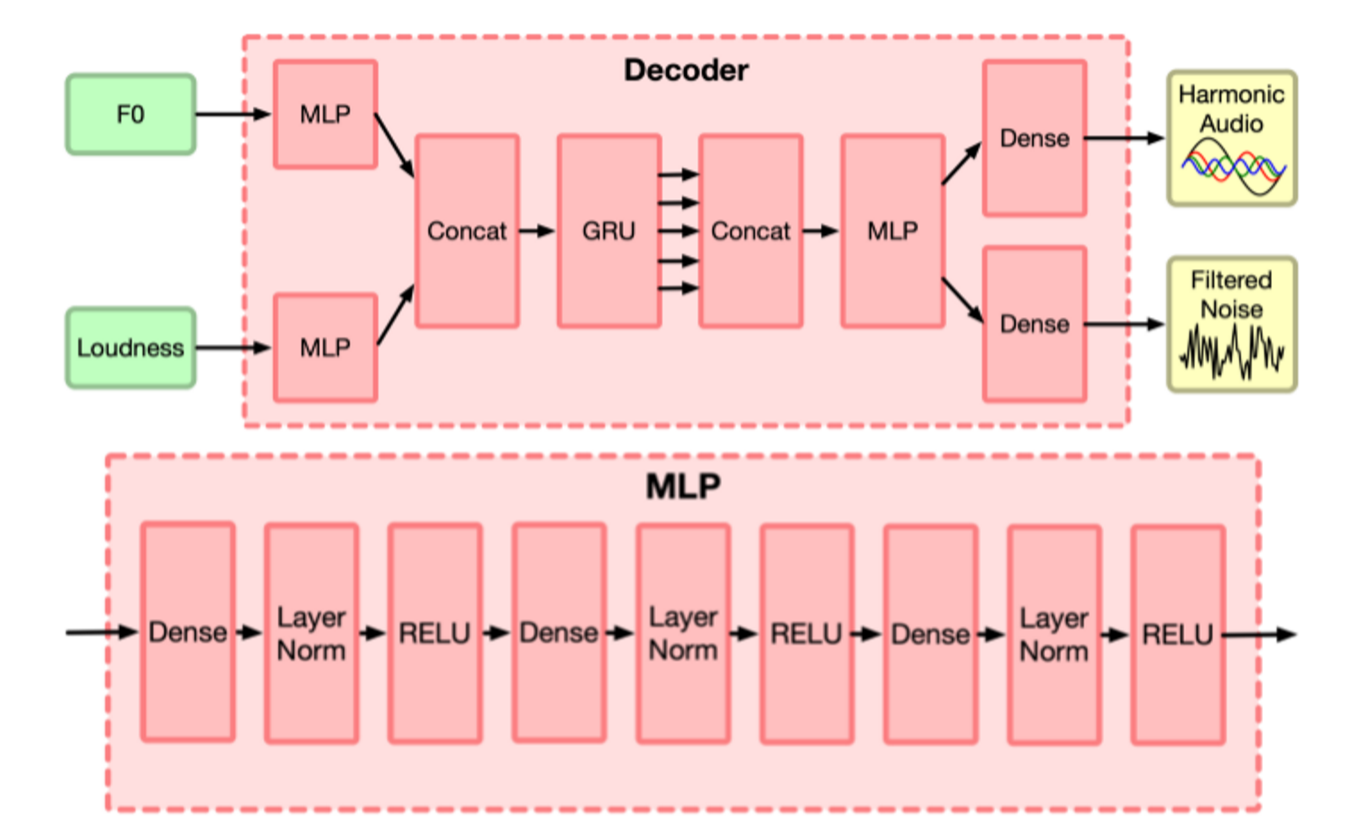
\includegraphics[width=0.8\textwidth]{literature_review/SingingDecoderMLP.png}
    \caption{Modified DDSP Decoder and MLP\cite{SingingDDSP}}
    \label{fig:singing_decoder_mlp}
\end{figure}

Even on a small dataset, promising results were obtained. Timbre transfer was possible. The performance of the modified decoder exceeded that of the original decoder.

Unfortunately, when the model was forced to recreate unseen sung lyrics, it was unintelligible, appearing to make stuttering noises. The model managed to obtain the correct loudness and pitch of the sound (except for the occasional pitch artefacts) but had no understanding of phonetics (i.e. the specific words that makeup speech). The paper suggests several steps for further work:

\begin{itemize}
    \item Phonetic condition of the model to model the nuances of human singing and to model the lyrics.
    \item Using synthesisers more suitable for modelling the human voice.
    \item Pre-processing of the fundamental frequency to remove pitch artefacts.
\end{itemize}

\subsection{DDSP Evaluation}

In the original paper, the DDSP decoder quickly learned how to re-synthesise datasets for a single instrument that sounded like the original audio sample.

A big pro of the method was that proper training on an instrument could be undertaken with as little as 15 minutes of training audio. Such a small dataset contrasts with models such as Jukebox, which require many hours of training audio as they are far larger models.

Due to the smaller model size, the model can operate with reduced training time and cost, making it more suitable for use in real-world applications and perhaps real-time applications.

Another plus was the interpretable and modular design of the model; individual factors such as pitch or loudness could be varied whilst keeping the others characteristics constant. This interpretation was possible because the model was conditioned to use pitch and loudness to re-synthesise the audio.

Additionally, individual components can be changed, perhaps without rebuilding the whole model. E.g. the spectrum based encoder can be replaced with a midi sourced encoder, with the rest of the model architecture remaining unchanged.

It was eventually decided that using the DDSP model would be picked for further research due to its modularity, accuracy and ease of use.

The variation of DDSP designed for \nameref{sec:singing_voice_synthesis} was chosen as this is a relatively novel area of research and held the most exciting applicability. However, this has historically proven to be a complex problem to solve. The human voice is not a simple harmonic series with a constant timbre.
\chapter{An Investigation in Using DDSP to Learn and Synthesize Vocal Features}

The adaptation of DDSP to synthesize vocal features such as singing using the additional MFFC layer was chosen for further investigation.

All research was undertaken using Google Colab notebooks and cloud hardware, primarily NVIDIA Tesla V100 GPUs.

Two seperate models were trained, one for a male voice (Chris Martin from Coldplay) and one for a female voice (Taylor Swift). This was done to see how the DDSP architecture would handle different vocies e.g. Alto or Tennor differently.

It was hypothesized that 2 albums would be the optimal size for any training dataset. Premilinary investigations on smaller datasets yielded significant overfitting and poor performance when any of the F0, amplitude latent features were modified during inference. Datasets of any greater size would be preferred. However, larger models would be slower to train.

\begin{figure}
    \centering
    \caption{Songs and albums going into each training dataset}
\end{figure}

\section{Dataset Preparation}

\subsection{Source Separation}

Following the selection of the two albums for each artist and removal of any songs where additional vocal artists to the main vocalist featured were removed, all songs were passed through the pre-trained Spleeter model\cite{SpleeterPip}\cite{SpleeterPip}. This pre-trained model can carry out source separation of instrumental and music tracks. Source separation was essential as the training dataset must not contain any instrumentals. The model outputted two separate tracks for each song, one representing the instrumentals and one the vocals. The instrumental tracks were discarded.

Using Spleeter to split existing songs with instrumental components opened up the possibility of using a more significant number of songs, something the original singing DDPS paper's authors did not consider. Their largest single voice dataset had a compressed size of ~70Mb, whereas the pre-processed datasets used in this paper were approximately ten times that at ~700Mb, whilst still being based on a single vocal artist, style of music, and vocals only tracks. Using a more extensive training dataset would reduce over-fitting and aid generalisation.

The remaining vocal tracks were then pre-processed.

\subsection{Pre-processing}

\begin{figure}[H]
    \centering
    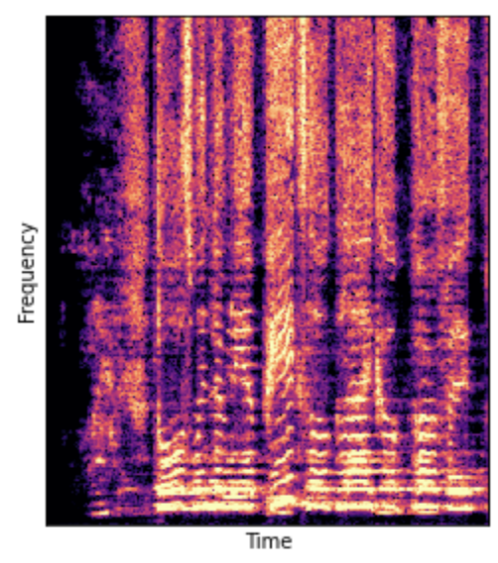
\includegraphics[width=0.6\textwidth]{research/dataset_preparation/PreprocessingSpecplot.png}
    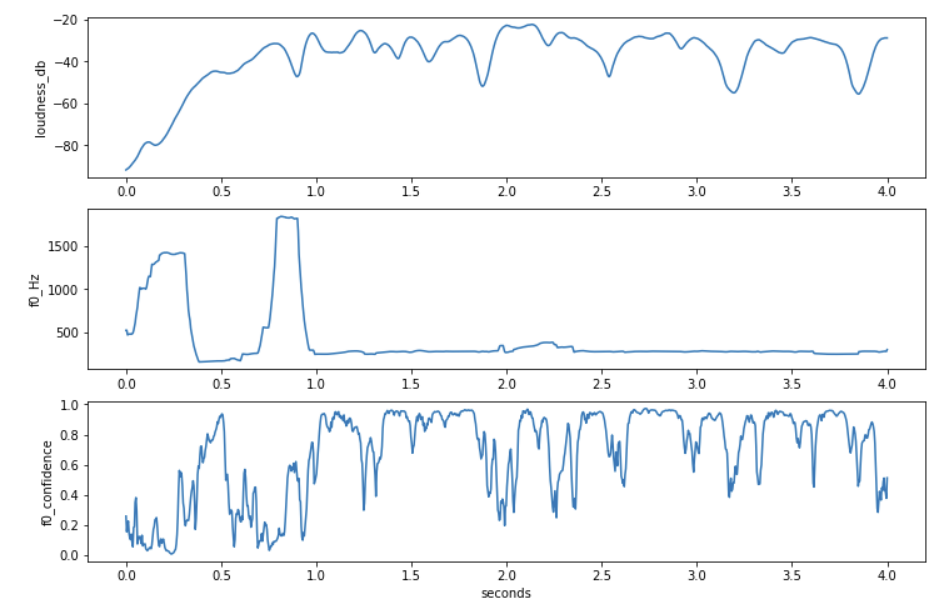
\includegraphics[width=0.8\textwidth]{research/dataset_preparation/PreprocessingFeatures.png}
    \caption{Dataset Pre-processing: Spectrogram plot of a random 4 second sample from one of the datasets and its accomanying F0, F0 Confidence and Amplitude characteristics over time throughout the sample}
\end{figure}

Pre-processing the datasets involved splitting the raw audio into smaller frames (samples), each 4 seconds long. The frame length was limited to 4 seconds to avoid capturing too much information in one spectrogram, which would make learning using the convolutional neural network difficult.

For each frame, F0 and confidence of F0 probability were inferred using CREPE\cite{CREPE}. Amplitude was computed statistically using the Librosa library\cite{LibrosaPip}. Latent Z information was available through the passing of the raw audio. The 4-second samples and accompanying features were then stored as TFRecord files.

Each of the two datasets was pre-processed on Google Colab notebooks; this process took approximately 40 minutes for each dataset using an NVIDIA Tesla V100 GPU.

Finally, a random 4-second clip was selected from each dataset to prove successful pre-processing. Its spectrogram was computed and plotted. Computed F0, F0 Confidence and Amplitude characteristics were also plotted for the selected clip. The underlying audio sample could also be played.

\section{Training}

A preprocessor was used that resampled the fundamental frequency and loudness, taking account the sample rate, frame rate, and number of timesteps. The number of timesteps was set at 1000 per 4 second clip, giving a spectral resoluiton of 4ms per timestep. This was deemed to be the best compromise between computational efficiency and accuracy.

An autoencoder encoder decoder setup was used. The encoder was based on Mfcc variant of a \acrfull{RNN}. The decoder was a RNN based decoder as described previously in \nameref{sec:singing_voice_synthesis}.

The model settings were kept the same as in \nameref{sec:singing_voice_synthesis} as they had already validated their hyperparameter selection. This included the use of100 sinusoidal harmonic components and 60 filter banks. This was done to limit model size to ensure it fitted on one GPU.

Each model was trained for 200,000 epochs, training time was approximately 2.9 epochs per second or 5.2 epochs per second depending on GPU used. Total training time was approxumately 20 horus per model.

\begin{figure}[!ht]
    \centering
    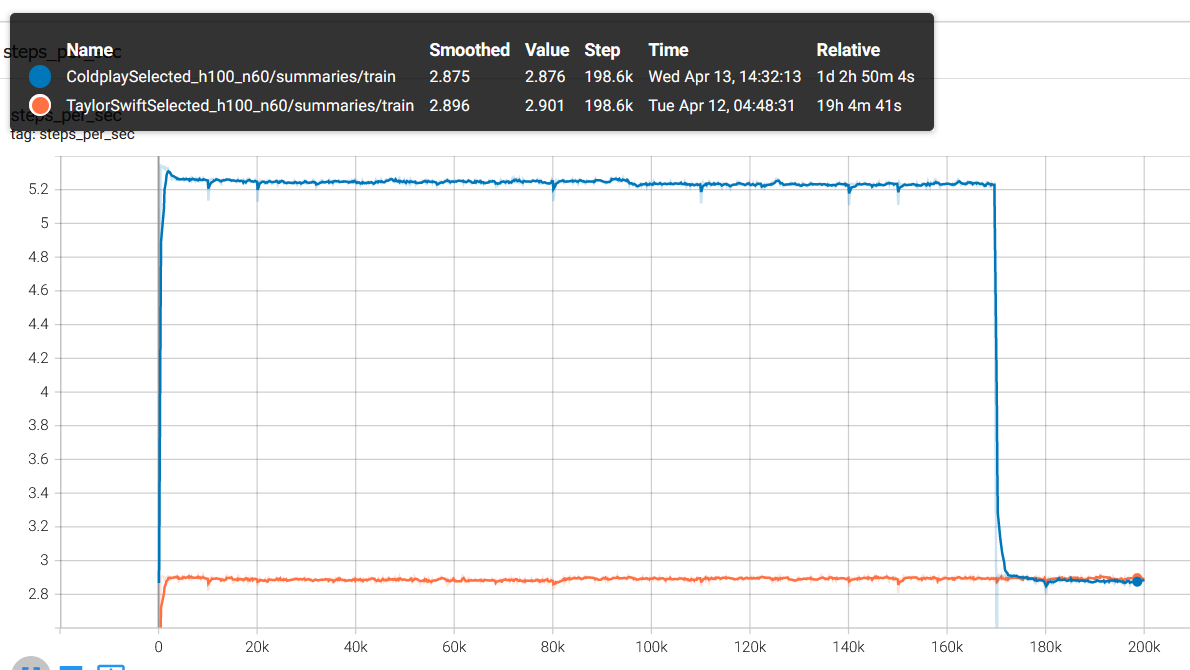
\includegraphics[width=0.6\textwidth]{research/training/StepsPerSecond.png}
    \caption{Training steps per second over the 200,000 training epochs}
\end{figure}

\begin{figure}[!ht]
    \centering
    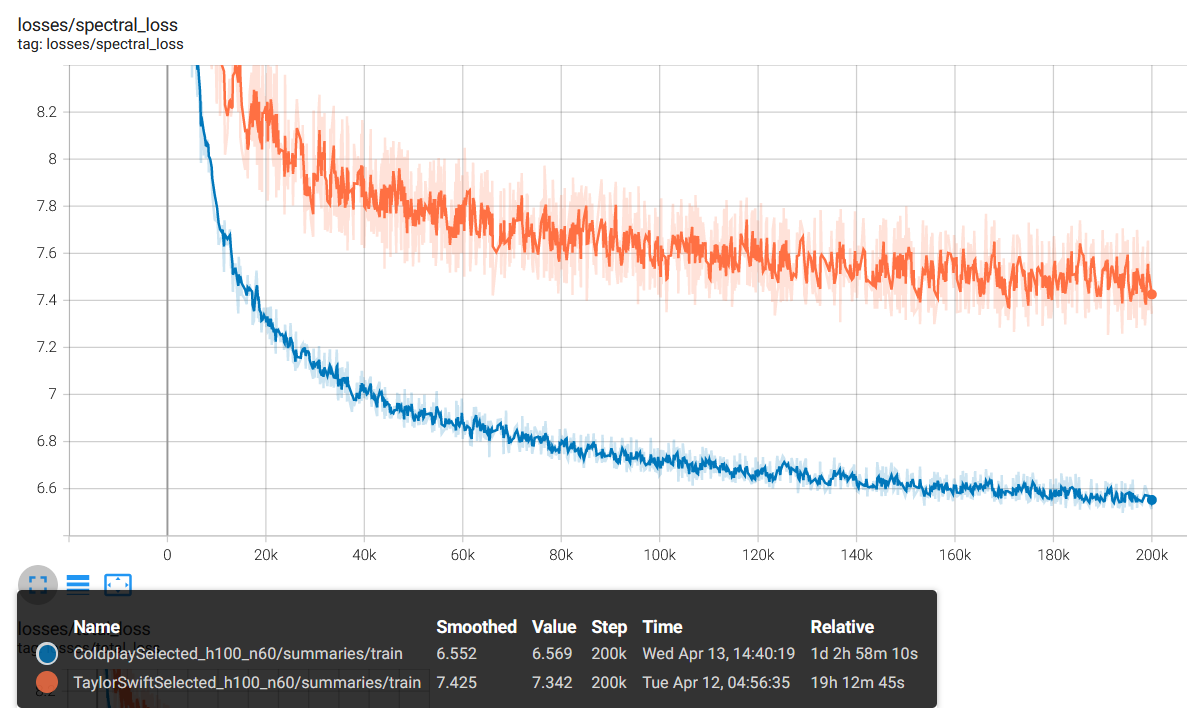
\includegraphics[width=0.8\textwidth]{research/training/TrainingSpectralLosses.png}
    \caption{Training Spectral Losses: Losses over the 200,000 epochs of training both models, using the spectral loss function defined in \nameref{sec:loss_measure}}
    \label{fig:training_spectral_losses}
\end{figure}

\nameref{fig:training_spectral_losses} shows the Coldplay losses being less than the Taylor Swift losses. This is due to the fact that the Coldplay Dataset having more frames that were pure silence, meaning that the Coldplay model fitted the silence frames more accurately.



\section{Results}

Several inferencing tests were conducted to see if the models had learned the latent features correctly to evaluate the models' performance.

All inferencing tests took approximately 0.3 seconds for a 4-minute frame; this is fast enough to enable real-time applications and significantly quicker than the Jukebox model.

\subsection{Recreation from the Training Dataset}

A random frame was selected and passed through each model; loudness and F0 were unmodified. The results of the inferencing were then compared to the original training dataset.

Each model successfully recreated original frames, though the Taylor Swift dataset yielded the best results.

Timbral features were slightly distorted (more so with the Coldplay model), but the overall quality was good, and it was easy to tell it was the original singer in both cases. In addition, pitch estimation was highly accurate and in line with the original pitch. Pitch accuracy can be partially attributed to the accuracy of the CREPE pitch detection model\cite{CREPE} and because the pitch was directly passed to the harmonic synthesiser.

The resynthesis of understandable words from the original frame was a far more considerable achievement. The original singing DDSP paper\cite{SingingDDSP} suffered a problem of stuttering when attempting resynthesis as their model was unable to recreate phonemes of the human voice accurately. It is possible that using far larger datasets has improved the quality of the resynthesis because the models had become more general in their ability to synthesise the human voice. However, it must be said that the Coldplay model was harder to understand.

\begin{figure}[H]
    \centering
    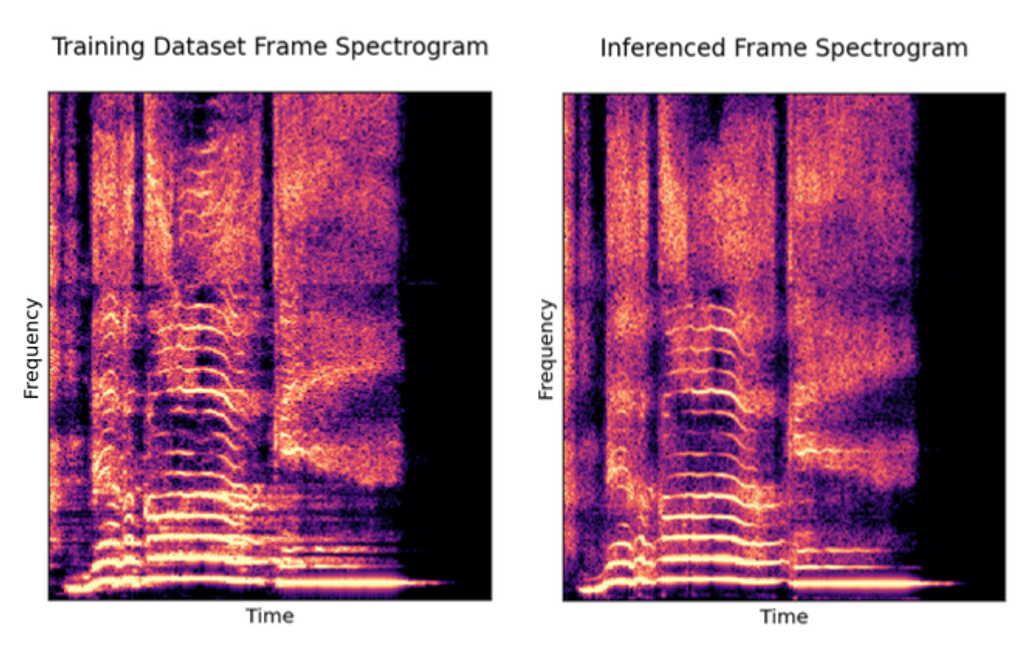
\includegraphics[width=0.8\textwidth]{research/results/TaylorSwift/InferredRecreation.png}
    \caption{(Taylor Swift) Original and resynthesized frames without latent modification}
\end{figure}

\begin{figure}[H]
    \centering
    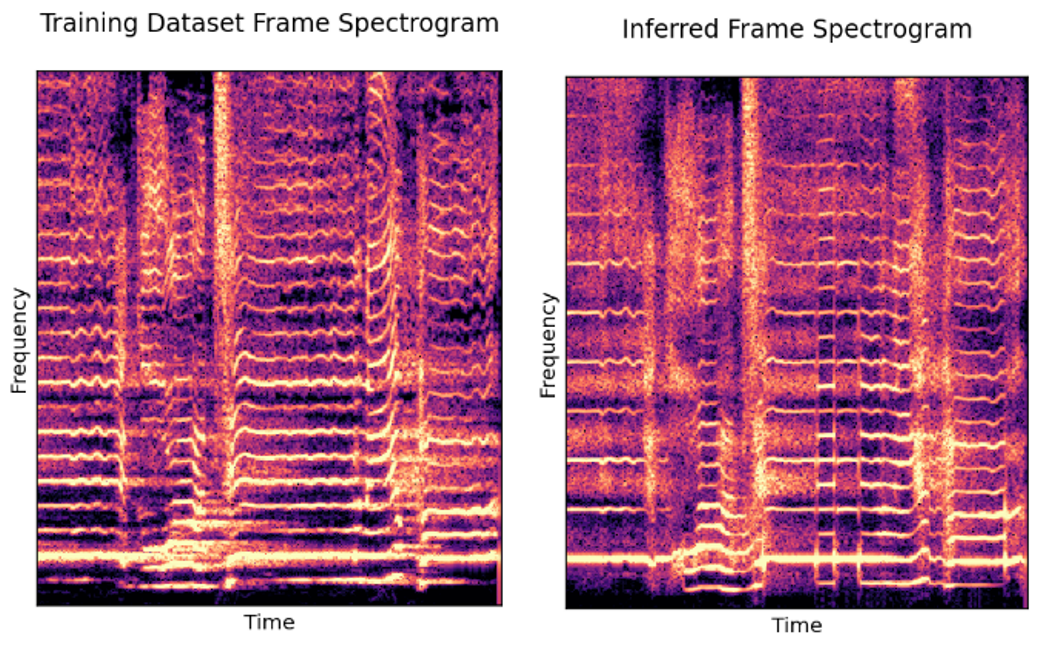
\includegraphics[width=0.8\textwidth]{research/results/Coldplay/InferredRecreation.png}
    \caption{(Coldplay) Original and resynthesized frames without latent modification}
\end{figure}

\subsection{F0 Pitch Transposition by a fixed octave}

A more advanced inferencing test was then undertaken. The fundamental frequency latent as determined by CREPE was transposed by fixed octaves (-2, -1, 0, 0.5, 1, 2), and the inferencing was re-performed on the transposed latents. Both models responded to the change in F0 and could accurately transpose harmonic pitch by the correct octave amount. At minor transpositions, e.g. +1 or -1 octave, the inferred frame still sounded somewhat like a human voice. However, it sounded like the noise, and harmonic components were separate sources at greater transpositions and did not constitute one voice.

As expected, modifying F0 did not change the pitch of the filtered noise at all, confirming that the pitch change had been directly passed to the harmonic synthesiser. This finding is interesting because we would have expected a little bit of distortion in the original pitch.

At extreme transpositions, harmonics sometimes appeared to go silent. The resynthesis sounded like a whisper, coming almost entirely out of the filtered noise. Whispering occurs when the vocal cords are held rigid, preventing them from vibrating and producing sinusoidal sounds (harmonics in the case of singing). The fact that the model's output sounded like a whisper is a good sign that the model was able to learn and distinguish the noise and harmonics as per the Harmonic Plus Noise Model\cite{HarmonicPlusNoise}\cite{OriginalDDSP}.

\begin{figure}[H]
    \centering
    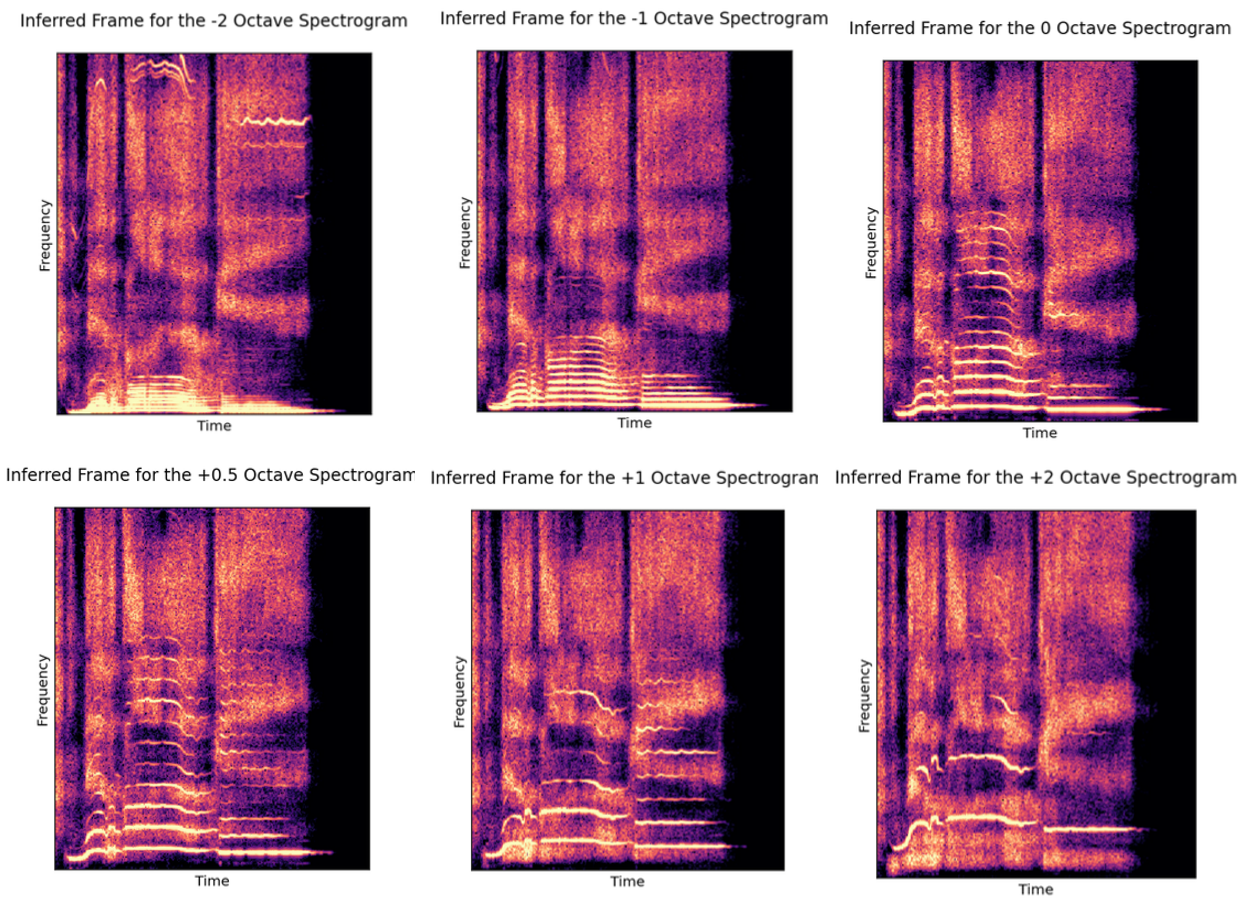
\includegraphics[width=\textwidth]{research/results/TaylorSwift/InferredTranspositions.png}
    \caption{(Taylor Swift) Inferred spectrogram frames at various octave transpositions realative to F0 at a certain timegrame in the original frame}
\end{figure}

\begin{figure}[H]
    \centering
    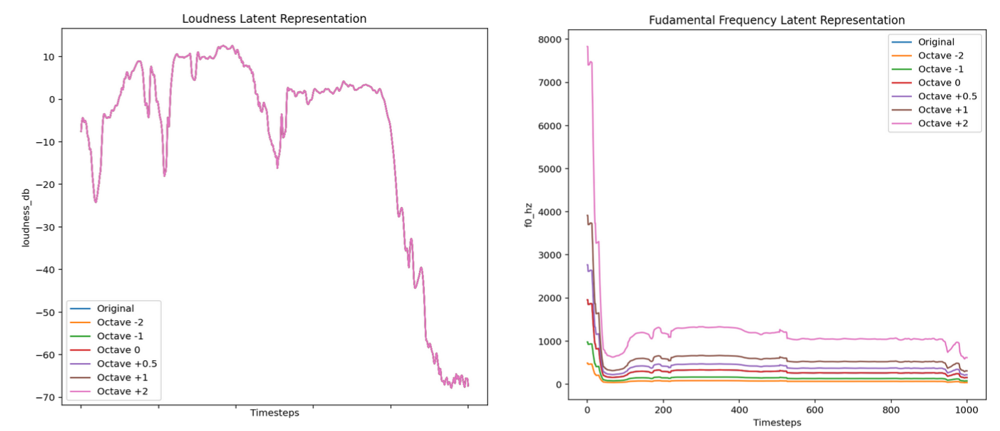
\includegraphics[width=\textwidth]{research/results/TaylorSwift/InferredTranspositionsGraphs.png}
    \caption{(Taylor Swift) Latent F0 and loudness features for various octave transpositions realative to F0 over timesteps throughout the frame}
\end{figure}

\begin{figure}[H]
    \centering
    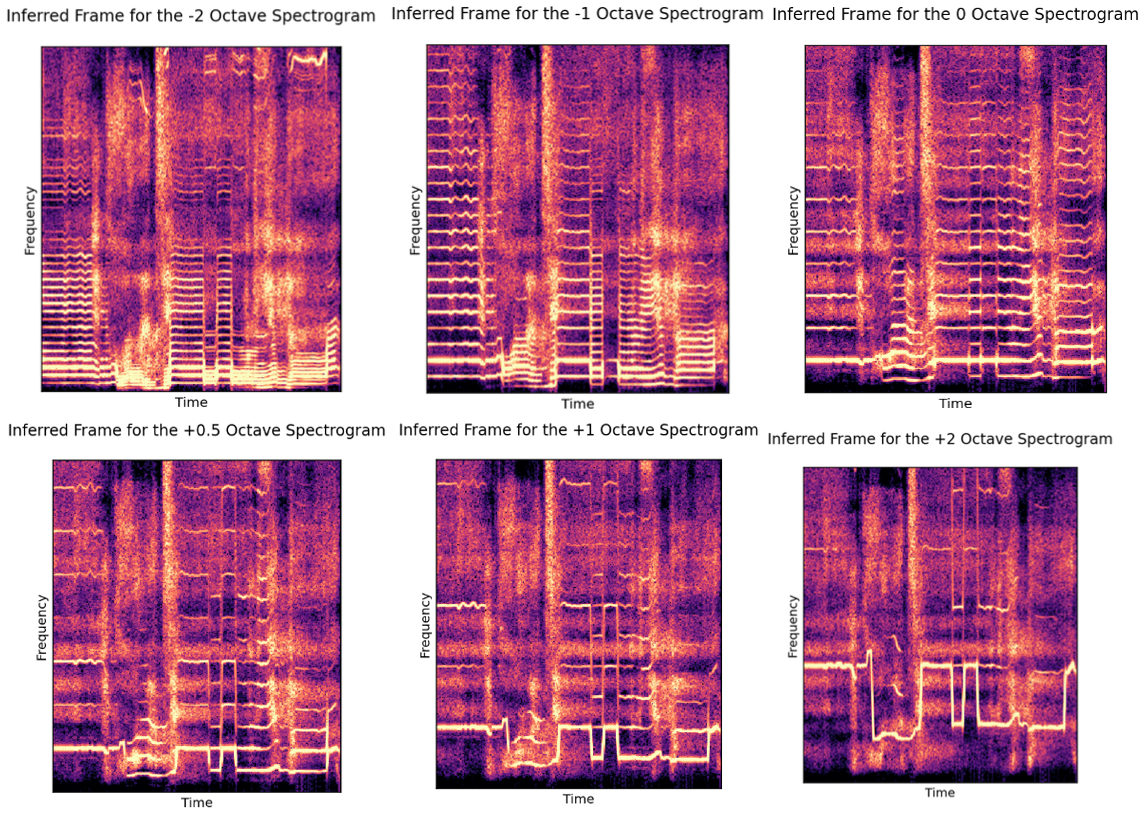
\includegraphics[width=\textwidth]{research/results/Coldplay/InferredTranspositions.png}
    \caption{(Coldplay) Inferred spectrogram frames at various octave transpositions realative to F0 at a certain timegrame in the original frame}
\end{figure}

\begin{figure}[H]
    \centering
    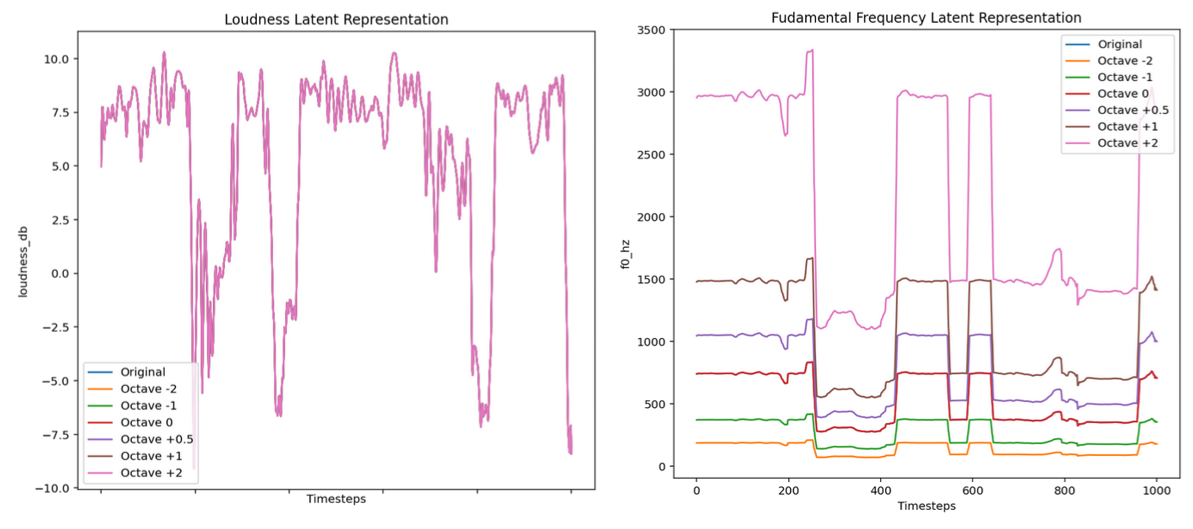
\includegraphics[width=\textwidth]{research/results/Coldplay/InferredTranspositionsGraphs.png}
    \caption{(Coldplay) Latent F0 and loudness features for various octave transpositions realative to F0 over timesteps throughout the frame}
\end{figure}

\subsection{Fixing F0}

The final pitch related test was fixing F0 to the mean value of F0 throughout the frame to see how the models would perform under unnatural pitch conditions.

Both models could fix the pitch to the mean value of F0 in the frame. This fixing is heard and can be seen visibly from the inferred spectrogram images where the harmonic components are at lines of constant frequency, unlike the original where they vary.

Additionally, words were still able to be synthesised and accurately heard, suggesting the model was able to learn the underlying phonemes of speech.

This result is excellent, mimicking what was founded in the speech DDSP research\cite{SpeechDDSP} (whose code was not publicly available). Further experiments were done with similar degrees of success in varying the pitch to other amounts, e.g. 100Hz and 500Hz. Again, however, the quality of results broke down at the extremes. The breakdown was evidenced by the harmonic again sounding more like a separate sound, with the whispers producing the actual words.

Sadly, timbral quality was reduced when F0 was fixed, with the output sounding more robotic and the original timbre being lost. Timbral loss is to be expected, however, as the original harmonic plus noise model was not designed with timbre transfer specifically in mind\cite{OriginalDDSP}.

\begin{figure}[H]
    \centering
    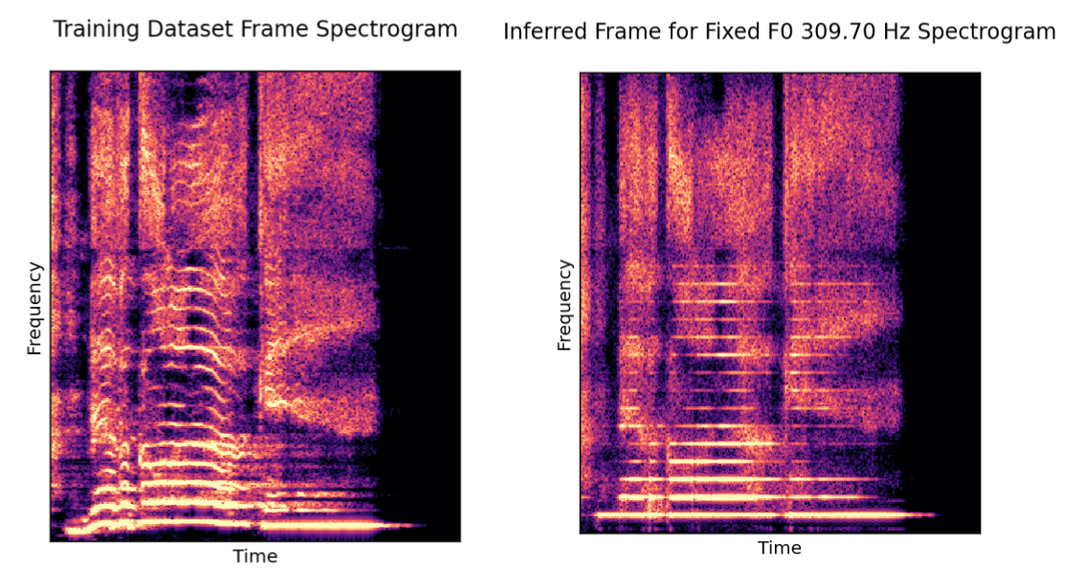
\includegraphics[width=\textwidth]{research/results/TaylorSwift/FixedF0.png}
    \caption{(Taylor Swift) Training dataset and fixed F0 spectrogram frames}
\end{figure}

\begin{figure}[H]
    \centering
    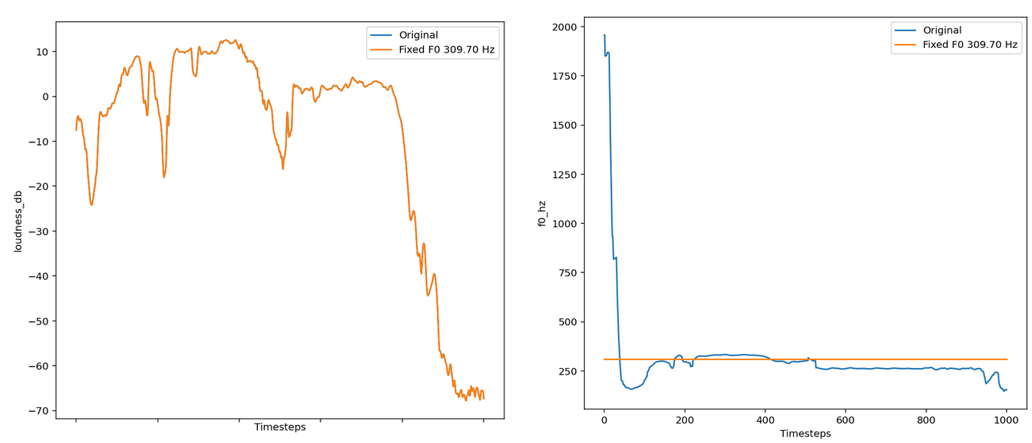
\includegraphics[width=\textwidth]{research/results/TaylorSwift/FixedF0Graphs.png}
    \caption{(Taylor Swift) Latent information on loudness and F0 over timesteps throughout the frame. The mean F0 was used to fix F0 throughout the frame}
\end{figure}

\begin{figure}[H]
    \centering
    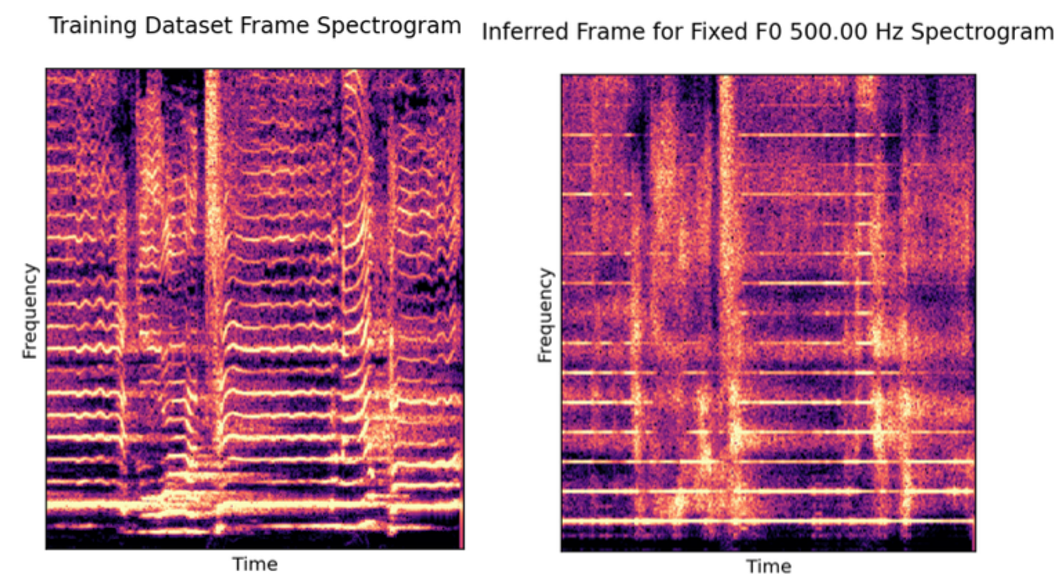
\includegraphics[width=\textwidth]{research/results/Coldplay/FixedF0.png}
    \caption{(Coldplay) Training dataset and fixed F0 spectrogram frames}
\end{figure}

\begin{figure}[H]
    \centering
    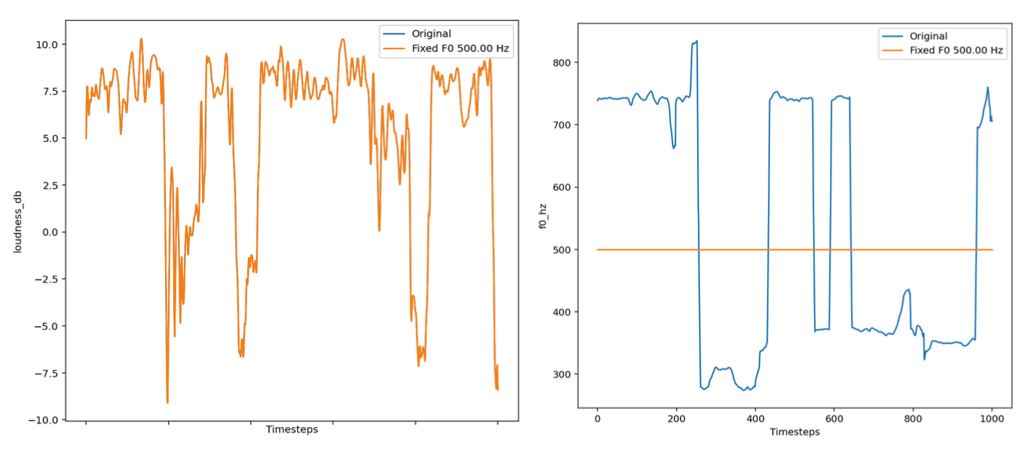
\includegraphics[width=\textwidth]{research/results/Coldplay/FixedF0Graphs.png}
    \caption{(Coldplay) Latent information on loudness and F0 over timesteps throughout the frame. The mean F0 was used to fix F0 throughout the frame}
\end{figure}

\subsection{Modifying Loudness}

Unfortunately, modification of the loudness latent vector did not alter the loudness of any inferred frames, and this could be caused by, perhaps, the decoder learning to ignore the latent loudness vector.

Alternatively, there may be some architectural issues with the modified decoder. For example, the DDSP library's authors significantly redesigned the loudness and power calculations with the version 3 release. Unfortunately, the Singing DDSP decoder used the older version 1. The discovery of any technical problems is beyond the scope of this thesis.

\subsection{Timbral Transfer}

The Taylor Swift model was selected for the timbral transfer tasks due to its better performance in the pitch transfer tests. For both male and female voice tests, vocals were successfully synthesised, and it was clear what words were being pronounced. Pitch was also accurately modelled for both cases. Success outside of the training set suggests that the model had successfully been generalised and had learned the underlying phonemes of human speech from spectrograms.

For the timbral transfer, the following songs were used:

\vspace{0.5cm}
\framebox[1.1\width]{
    \begin{minipage}{0.8\textwidth}
        \begin{itemize}
            \item \textbf{(Male Voice) Lewis Capaldi - \textit{Someone You Loved}}
            \item \textbf{(Female Voice) Birdy - \textit{Deep End}}
        \end{itemize}
    \end{minipage}
}
\vspace{0.5cm}

Sadly, the timbral transfer did not occur, with each inferred frame sounding similar to the source artist and not that of the training dataset. This result suggests that the model had learned to transfer timbre from the original vocal frame to the synthesised frame. Timbral quality was also reduced, sounding more unnatural, suggesting that perfect generalisation was not fully achieved. 

\begin{figure}[H]
    \centering
    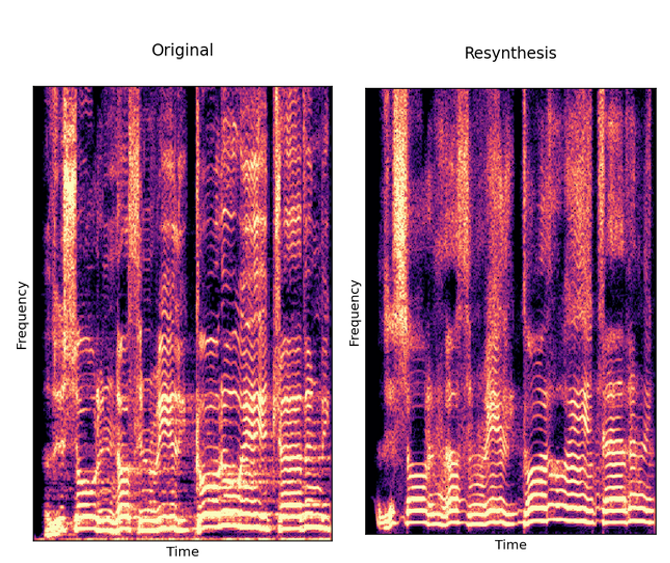
\includegraphics[width=\textwidth]{research/results/LewisCapaldi/TimbralTransfer.png}
    \caption{Lewis Capaldi timbral transfer test showing a comparison between the orignal and infererd spectrogram frames using the Taylor Swift model}
\end{figure}

\begin{figure}[H]
    \centering
    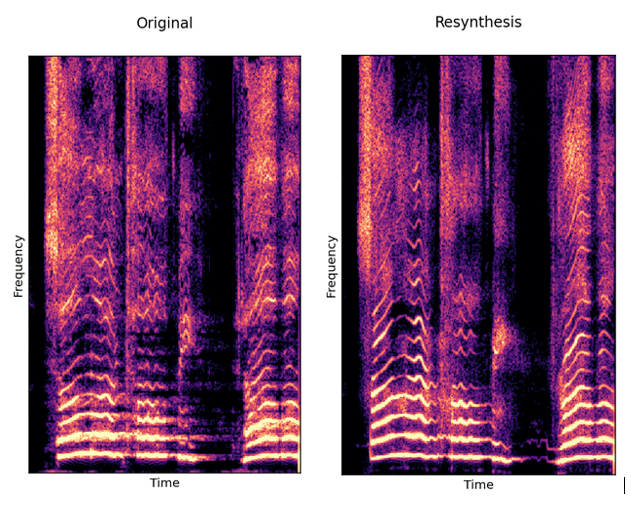
\includegraphics[width=\textwidth]{research/results/Birdy/TimbralTransfer.png}
    \caption{Birdy timbral transfer test showing a comparison between the oriignal and infererd spectrogram frames using the Taylor Swift model}
\end{figure}

\subsection{Inference with Instrumentals}

The Taylor Swift model was then used to infer a frame featuring the instrumental and vocal version of the song Deep End (i.e. the original song before passing through the Spleeter model).

The DDSP model managed to extract vocals from the track with instrumentals. Even more significant, there was no leakage of instrumentals in the inferred frame, suggesting that the model had isolated features unique to the human voice instead of more general noise features.

This result shows that the DDSP model is very flexible, being able to carry out source separation tasks similar to the Spleeter library\cite{Spleeter}; this was not demonstrated in the previous DDSP papers.

The inferred frames from the tracks with and without instrumentals sounded similar; however, F0 estimation in the frame with instrumentals could be better. Inaccurate F0 estimation is likely a limitation of using CREPE pitch estimation on a track with multiple parts simultaneously.

\begin{figure}[H]
    \centering
    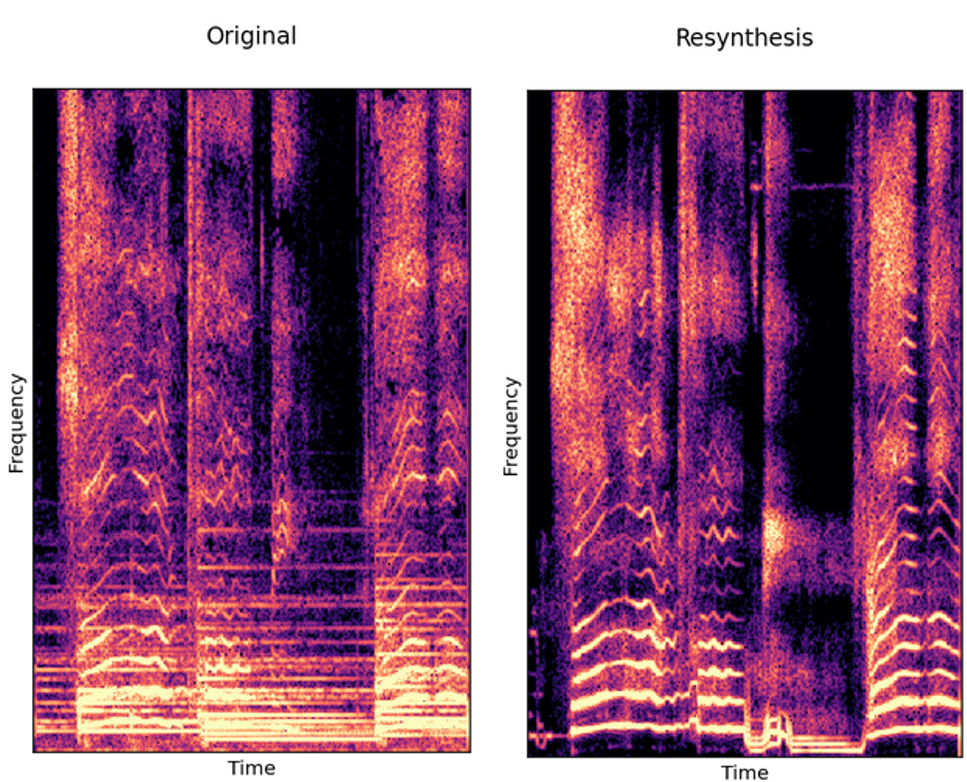
\includegraphics[width=\textwidth]{research/results/Birdy/InferenceWithInstrumentals.png}
    \caption{Birdy instrumental and vocals inference test using the Taylor Swift model, showing the original and infered spectrogram frames}
\end{figure}

\subsection{General Problems}

Along with the loudness perception problem, others were encountered during all inferencing tests:

\begin{enumerate}
    \item At low loudness levels, the CREPE model could not accurately detect the pitch of the audio sample. This lack of accuracy caused the fundamental frequency to jump around, sometimes appearing to jump up or down an octave, making the output sound jarring; this is evidenced in the Coldplay frames that all experience this problem. The DDSP authors suggested a potential solution was muting sections of the track where CREPE had low confidence in its prediction. Sadly, this fix could not work here due to the problems discussed around the loudness latent.
    \item The models failed to learn specific timbre related to the trained artist; this was especially apparent during the constant F0 test when the output sounded almost robotic. Lack of timbre transfer was foreseen as the DDSP architecture was not directly designed for timbre transfer.
    \item Similarly, when transferring timbre from another artist, the inferred sample sounded like the voice of the other artist more than it did that of the training dataset artist. However, this result could be attributed to the model's generalisation to synthesise the specific timbres derived from the noise characteristics of a test frame.
\end{enumerate}

The failure to learn timbre, as demonstrated throughout all the tests, could be the price paid for the ability of the model to understand, interpret, and synthesise any given voice.
\chapter{Conclusions and Reccomendations}

\section{Experimental Conclusions}

In summary, DDSP has demonstrated itself as a very powerful tool for learning and synthesizing vocal features of the human voice. The experiments shown in this paper how it was able to learn how to accurately infer pitch and phoentic information about the human voice. This is significant as it appears to overcome the problems of the original MFCC DDSP model\cite{SingingDDSP} which was unable to learn the underlying phonemes of speech and produce coherent speech.

It could be said that despite the failure of the models in this paper to trasnfer timbre and loudness, the interpretable pitch feature of DDSP has been successfilly learned and demonstrated in a variety of sitations that demonstate genarability outside of the training dataset.

Further applicability previously not explored in the DDSP paper, such as vocal source separation has also been demonstrated. This is due to the fact that the model had successfully learned to infer the vocal source from the audio signal.

DDSP will have a future in synthesing realistic music vocals and could be used for further accademic or artistic purposes. Its interpretable and modular nature will allow it to be integrated into other applications.

\section{Reccomendations}

There are however many areas of improvement that can be made to the model. Firstly, accurate loudness estimation must be implemented, this is a feature of the original DDSP model\cite{OriginalDDSP} that appears to not be working with the variation applied to singing. This may require an extensive review of the decoder to ensure it is programmed correctly. If it is found to be working, then the loss function may have to be altered to bias the model towards the amplitude latent vector.

The timbral quality although good could be better, this could be improved by increasing the number of internal parameters and increasing the resolution of spectrogtrams used. This change would increase model size significantly requiring its parellizaiton and training on multiple GPUs.

Future works could focus on implementing DDSP with other technologies and machine learning models. A DDSP based model could be combined with an attention based symbolic transformer model, natural langauge model such as GPT-3\cite{GPT3} and text to speech systems to provide an end to end program that could generate a whole song. The symbolic transformer model could generate long term features such as F0 over time (in the form of midi notation) as well as other long term musical features and characteristics. The natural language model could then be tasked with generating lyrics to match the timings of the generated music. These could be synthesized using text to speech and F0 or other characteristics modified by DDSP.

% This ensures that the subsequent sections are being included as root
% items in the bookmark structure of your PDF reader.
\bookmarksetup{startatroot}
\backmatter

\begingroup
\let\clearpage\relax
\glsaddall
\printglossary[type=\acronymtype]
\newpage
\printglossary
\endgroup

\chapter{Open Source Licenses}
\label{chapter:open_source_licenses}

\begin{enumerate}
    \item Latex Mimososis Latex Template\cite{LatexMimosis}
    \item DDSP (Differentiable Digital Signal Processing) Python Library\cite{DDSPPip}
    \item Spleeter - Source Separation Library\cite{SpleeterPip}
\end{enumerate}

\printindex
\printbibliography

\end{document}
